\documentclass{standalone}
\usepackage{tikz}
\begin{document}
% Created by tikzDevice version 0.7.0 on 2015-04-25 22:09:43
% !TEX encoding = UTF-8 Unicode
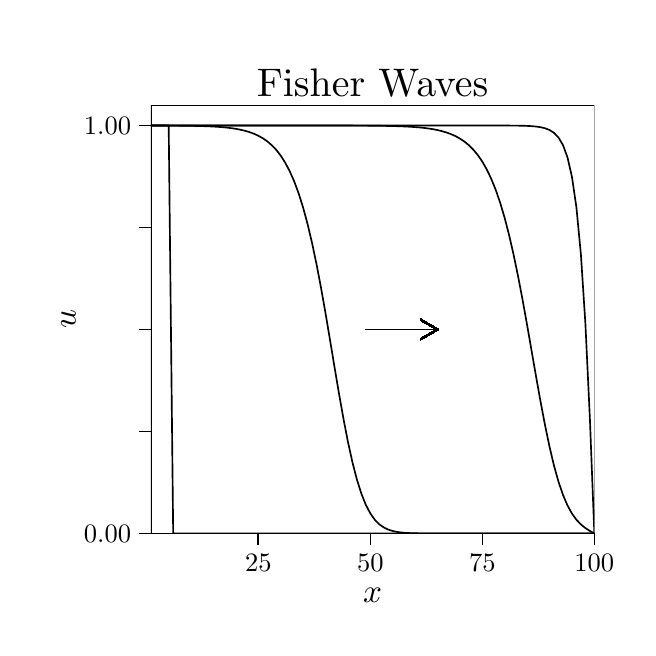
\begin{tikzpicture}[x=1pt,y=1pt]
\definecolor[named]{fillColor}{rgb}{1.00,1.00,1.00}
\path[use as bounding box,fill=fillColor,fill opacity=0.00] (0,0) rectangle (216.81,216.81);
\begin{scope}
\path[clip] (  0.00,  0.00) rectangle (216.81,216.81);
\definecolor[named]{drawColor}{rgb}{1.00,1.00,1.00}
\definecolor[named]{fillColor}{rgb}{1.00,1.00,1.00}

\path[draw=drawColor,line width= 0.6pt,line join=round,line cap=round,fill=fillColor] ( -0.00,  0.00) rectangle (216.81,216.81);
\end{scope}
\begin{scope}
\path[clip] ( 44.49, 34.03) rectangle (204.76,188.82);
\definecolor[named]{fillColor}{rgb}{1.00,1.00,1.00}

\path[fill=fillColor] ( 44.49, 34.03) rectangle (204.76,188.82);
\definecolor[named]{drawColor}{rgb}{0.00,0.00,0.00}

\path[draw=drawColor,line width= 0.6pt,line join=round] ( 44.49,181.45) --
	( 46.10,181.45) --
	( 47.72,181.45) --
	( 49.34,181.45) --
	( 50.96,181.45) --
	( 52.58, 34.03) --
	( 54.20, 34.03) --
	( 55.82, 34.03) --
	( 57.44, 34.03) --
	( 59.06, 34.03) --
	( 60.68, 34.03) --
	( 62.29, 34.03) --
	( 63.91, 34.03) --
	( 65.53, 34.03) --
	( 67.15, 34.03) --
	( 68.77, 34.03) --
	( 70.39, 34.03) --
	( 72.01, 34.03) --
	( 73.63, 34.03) --
	( 75.25, 34.03) --
	( 76.87, 34.03) --
	( 78.48, 34.03) --
	( 80.10, 34.03) --
	( 81.72, 34.03) --
	( 83.34, 34.03) --
	( 84.96, 34.03) --
	( 86.58, 34.03) --
	( 88.20, 34.03) --
	( 89.82, 34.03) --
	( 91.44, 34.03) --
	( 93.05, 34.03) --
	( 94.67, 34.03) --
	( 96.29, 34.03) --
	( 97.91, 34.03) --
	( 99.53, 34.03) --
	(101.15, 34.03) --
	(102.77, 34.03) --
	(104.39, 34.03) --
	(106.01, 34.03) --
	(107.63, 34.03) --
	(109.24, 34.03) --
	(110.86, 34.03) --
	(112.48, 34.03) --
	(114.10, 34.03) --
	(115.72, 34.03) --
	(117.34, 34.03) --
	(118.96, 34.03) --
	(120.58, 34.03) --
	(122.20, 34.03) --
	(123.82, 34.03) --
	(125.43, 34.03) --
	(127.05, 34.03) --
	(128.67, 34.03) --
	(130.29, 34.03) --
	(131.91, 34.03) --
	(133.53, 34.03) --
	(135.15, 34.03) --
	(136.77, 34.03) --
	(138.39, 34.03) --
	(140.01, 34.03) --
	(141.62, 34.03) --
	(143.24, 34.03) --
	(144.86, 34.03) --
	(146.48, 34.03) --
	(148.10, 34.03) --
	(149.72, 34.03) --
	(151.34, 34.03) --
	(152.96, 34.03) --
	(154.58, 34.03) --
	(156.20, 34.03) --
	(157.81, 34.03) --
	(159.43, 34.03) --
	(161.05, 34.03) --
	(162.67, 34.03) --
	(164.29, 34.03) --
	(165.91, 34.03) --
	(167.53, 34.03) --
	(169.15, 34.03) --
	(170.77, 34.03) --
	(172.39, 34.03) --
	(174.00, 34.03) --
	(175.62, 34.03) --
	(177.24, 34.03) --
	(178.86, 34.03) --
	(180.48, 34.03) --
	(182.10, 34.03) --
	(183.72, 34.03) --
	(185.34, 34.03) --
	(186.96, 34.03) --
	(188.58, 34.03) --
	(190.19, 34.03) --
	(191.81, 34.03) --
	(193.43, 34.03) --
	(195.05, 34.03) --
	(196.67, 34.03) --
	(198.29, 34.03) --
	(199.91, 34.03) --
	(201.53, 34.03) --
	(203.15, 34.03) --
	(204.76, 34.03);

\path[draw=drawColor,line width= 0.6pt,line join=round] ( 44.49,181.45) --
	( 46.10,181.44) --
	( 47.72,181.44) --
	( 49.34,181.43) --
	( 50.96,181.42) --
	( 52.58,181.41) --
	( 54.20,181.40) --
	( 55.82,181.38) --
	( 57.44,181.36) --
	( 59.06,181.34) --
	( 60.68,181.30) --
	( 62.29,181.26) --
	( 63.91,181.21) --
	( 65.53,181.15) --
	( 67.15,181.07) --
	( 68.77,180.97) --
	( 70.39,180.85) --
	( 72.01,180.69) --
	( 73.63,180.49) --
	( 75.25,180.25) --
	( 76.87,179.94) --
	( 78.48,179.56) --
	( 80.10,179.09) --
	( 81.72,178.49) --
	( 83.34,177.76) --
	( 84.96,176.85) --
	( 86.58,175.73) --
	( 88.20,174.35) --
	( 89.82,172.65) --
	( 91.44,170.57) --
	( 93.05,168.04) --
	( 94.67,164.98) --
	( 96.29,161.31) --
	( 97.91,156.94) --
	( 99.53,151.79) --
	(101.15,145.81) --
	(102.77,138.96) --
	(104.39,131.25) --
	(106.01,122.75) --
	(107.63,113.60) --
	(109.24,104.01) --
	(110.86, 94.26) --
	(112.48, 84.66) --
	(114.10, 75.54) --
	(115.72, 67.18) --
	(117.34, 59.81) --
	(118.96, 53.54) --
	(120.58, 48.42) --
	(122.20, 44.37) --
	(123.82, 41.28) --
	(125.43, 39.00) --
	(127.05, 37.36) --
	(128.67, 36.22) --
	(130.29, 35.44) --
	(131.91, 34.93) --
	(133.53, 34.59) --
	(135.15, 34.38) --
	(136.77, 34.24) --
	(138.39, 34.16) --
	(140.01, 34.11) --
	(141.62, 34.08) --
	(143.24, 34.06) --
	(144.86, 34.05) --
	(146.48, 34.04) --
	(148.10, 34.04) --
	(149.72, 34.04) --
	(151.34, 34.04) --
	(152.96, 34.04) --
	(154.58, 34.03) --
	(156.20, 34.03) --
	(157.81, 34.03) --
	(159.43, 34.03) --
	(161.05, 34.03) --
	(162.67, 34.03) --
	(164.29, 34.03) --
	(165.91, 34.03) --
	(167.53, 34.03) --
	(169.15, 34.03) --
	(170.77, 34.03) --
	(172.39, 34.03) --
	(174.00, 34.03) --
	(175.62, 34.03) --
	(177.24, 34.03) --
	(178.86, 34.03) --
	(180.48, 34.03) --
	(182.10, 34.03) --
	(183.72, 34.03) --
	(185.34, 34.03) --
	(186.96, 34.03) --
	(188.58, 34.03) --
	(190.19, 34.03) --
	(191.81, 34.03) --
	(193.43, 34.03) --
	(195.05, 34.03) --
	(196.67, 34.03) --
	(198.29, 34.03) --
	(199.91, 34.03) --
	(201.53, 34.03) --
	(203.15, 34.03) --
	(204.76, 34.03);

\path[draw=drawColor,line width= 0.6pt,line join=round] ( 44.49,181.45) --
	( 46.10,181.45) --
	( 47.72,181.45) --
	( 49.34,181.45) --
	( 50.96,181.45) --
	( 52.58,181.45) --
	( 54.20,181.45) --
	( 55.82,181.45) --
	( 57.44,181.45) --
	( 59.06,181.45) --
	( 60.68,181.45) --
	( 62.29,181.45) --
	( 63.91,181.45) --
	( 65.53,181.45) --
	( 67.15,181.45) --
	( 68.77,181.45) --
	( 70.39,181.45) --
	( 72.01,181.45) --
	( 73.63,181.45) --
	( 75.25,181.45) --
	( 76.87,181.45) --
	( 78.48,181.45) --
	( 80.10,181.45) --
	( 81.72,181.45) --
	( 83.34,181.45) --
	( 84.96,181.45) --
	( 86.58,181.45) --
	( 88.20,181.45) --
	( 89.82,181.45) --
	( 91.44,181.45) --
	( 93.05,181.45) --
	( 94.67,181.45) --
	( 96.29,181.45) --
	( 97.91,181.45) --
	( 99.53,181.45) --
	(101.15,181.45) --
	(102.77,181.45) --
	(104.39,181.45) --
	(106.01,181.45) --
	(107.63,181.45) --
	(109.24,181.44) --
	(110.86,181.44) --
	(112.48,181.44) --
	(114.10,181.44) --
	(115.72,181.43) --
	(117.34,181.43) --
	(118.96,181.42) --
	(120.58,181.41) --
	(122.20,181.40) --
	(123.82,181.39) --
	(125.43,181.37) --
	(127.05,181.35) --
	(128.67,181.33) --
	(130.29,181.29) --
	(131.91,181.26) --
	(133.53,181.21) --
	(135.15,181.15) --
	(136.77,181.08) --
	(138.39,180.99) --
	(140.01,180.88) --
	(141.62,180.75) --
	(143.24,180.58) --
	(144.86,180.37) --
	(146.48,180.12) --
	(148.10,179.80) --
	(149.72,179.41) --
	(151.34,178.93) --
	(152.96,178.34) --
	(154.58,177.62) --
	(156.20,176.74) --
	(157.81,175.65) --
	(159.43,174.33) --
	(161.05,172.71) --
	(162.67,170.76) --
	(164.29,168.39) --
	(165.91,165.55) --
	(167.53,162.16) --
	(169.15,158.14) --
	(170.77,153.43) --
	(172.39,147.96) --
	(174.00,141.69) --
	(175.62,134.62) --
	(177.24,126.79) --
	(178.86,118.29) --
	(180.48,109.29) --
	(182.10, 99.99) --
	(183.72, 90.67) --
	(185.34, 81.60) --
	(186.96, 73.08) --
	(188.58, 65.33) --
	(190.19, 58.52) --
	(191.81, 52.74) --
	(193.43, 47.98) --
	(195.05, 44.19) --
	(196.67, 41.24) --
	(198.29, 39.00) --
	(199.91, 37.30) --
	(201.53, 36.00) --
	(203.15, 34.95) --
	(204.76, 34.03);

\path[draw=drawColor,line width= 0.6pt,line join=round] ( 44.49,181.45) --
	( 46.10,181.45) --
	( 47.72,181.45) --
	( 49.34,181.45) --
	( 50.96,181.45) --
	( 52.58,181.45) --
	( 54.20,181.45) --
	( 55.82,181.45) --
	( 57.44,181.45) --
	( 59.06,181.45) --
	( 60.68,181.45) --
	( 62.29,181.45) --
	( 63.91,181.45) --
	( 65.53,181.45) --
	( 67.15,181.45) --
	( 68.77,181.45) --
	( 70.39,181.45) --
	( 72.01,181.45) --
	( 73.63,181.45) --
	( 75.25,181.45) --
	( 76.87,181.45) --
	( 78.48,181.45) --
	( 80.10,181.45) --
	( 81.72,181.45) --
	( 83.34,181.45) --
	( 84.96,181.45) --
	( 86.58,181.45) --
	( 88.20,181.45) --
	( 89.82,181.45) --
	( 91.44,181.45) --
	( 93.05,181.45) --
	( 94.67,181.45) --
	( 96.29,181.45) --
	( 97.91,181.45) --
	( 99.53,181.45) --
	(101.15,181.45) --
	(102.77,181.45) --
	(104.39,181.45) --
	(106.01,181.45) --
	(107.63,181.45) --
	(109.24,181.45) --
	(110.86,181.45) --
	(112.48,181.45) --
	(114.10,181.45) --
	(115.72,181.45) --
	(117.34,181.45) --
	(118.96,181.45) --
	(120.58,181.45) --
	(122.20,181.45) --
	(123.82,181.45) --
	(125.43,181.45) --
	(127.05,181.45) --
	(128.67,181.45) --
	(130.29,181.45) --
	(131.91,181.45) --
	(133.53,181.45) --
	(135.15,181.45) --
	(136.77,181.45) --
	(138.39,181.45) --
	(140.01,181.45) --
	(141.62,181.45) --
	(143.24,181.45) --
	(144.86,181.45) --
	(146.48,181.45) --
	(148.10,181.45) --
	(149.72,181.45) --
	(151.34,181.45) --
	(152.96,181.45) --
	(154.58,181.45) --
	(156.20,181.45) --
	(157.81,181.45) --
	(159.43,181.45) --
	(161.05,181.45) --
	(162.67,181.45) --
	(164.29,181.45) --
	(165.91,181.45) --
	(167.53,181.45) --
	(169.15,181.45) --
	(170.77,181.45) --
	(172.39,181.44) --
	(174.00,181.43) --
	(175.62,181.42) --
	(177.24,181.40) --
	(178.86,181.37) --
	(180.48,181.31) --
	(182.10,181.22) --
	(183.72,181.08) --
	(185.34,180.84) --
	(186.96,180.46) --
	(188.58,179.83) --
	(190.19,178.79) --
	(191.81,177.11) --
	(193.43,174.38) --
	(195.05,169.97) --
	(196.67,162.92) --
	(198.29,151.83) --
	(199.91,134.82) --
	(201.53,109.85) --
	(203.15, 75.67) --
	(204.76, 34.03);
\definecolor[named]{fillColor}{rgb}{0.00,0.00,0.00}

\path[draw=drawColor,line width= 0.6pt,line join=round,fill=fillColor] (122.20,107.74) -- (148.10,107.74);

\path[draw=drawColor,line width= 0.6pt,line join=round] (141.94,104.19) --
	(148.10,107.74) --
	(141.94,111.30);

\path[draw=drawColor,line width= 0.6pt,line join=round,fill=fillColor] (122.20,107.74) -- (148.10,107.74);

\path[draw=drawColor,line width= 0.6pt,line join=round] (141.94,104.19) --
	(148.10,107.74) --
	(141.94,111.30);

\path[draw=drawColor,line width= 0.6pt,line join=round,fill=fillColor] (122.20,107.74) -- (148.10,107.74);

\path[draw=drawColor,line width= 0.6pt,line join=round] (141.94,104.19) --
	(148.10,107.74) --
	(141.94,111.30);

\path[draw=drawColor,line width= 0.6pt,line join=round,fill=fillColor] (122.20,107.74) -- (148.10,107.74);

\path[draw=drawColor,line width= 0.6pt,line join=round] (141.94,104.19) --
	(148.10,107.74) --
	(141.94,111.30);

\path[draw=drawColor,line width= 0.6pt,line join=round,fill=fillColor] (122.20,107.74) -- (148.10,107.74);

\path[draw=drawColor,line width= 0.6pt,line join=round] (141.94,104.19) --
	(148.10,107.74) --
	(141.94,111.30);

\path[draw=drawColor,line width= 0.6pt,line join=round,fill=fillColor] (122.20,107.74) -- (148.10,107.74);

\path[draw=drawColor,line width= 0.6pt,line join=round] (141.94,104.19) --
	(148.10,107.74) --
	(141.94,111.30);

\path[draw=drawColor,line width= 0.6pt,line join=round,fill=fillColor] (122.20,107.74) -- (148.10,107.74);

\path[draw=drawColor,line width= 0.6pt,line join=round] (141.94,104.19) --
	(148.10,107.74) --
	(141.94,111.30);

\path[draw=drawColor,line width= 0.6pt,line join=round,fill=fillColor] (122.20,107.74) -- (148.10,107.74);

\path[draw=drawColor,line width= 0.6pt,line join=round] (141.94,104.19) --
	(148.10,107.74) --
	(141.94,111.30);

\path[draw=drawColor,line width= 0.6pt,line join=round,fill=fillColor] (122.20,107.74) -- (148.10,107.74);

\path[draw=drawColor,line width= 0.6pt,line join=round] (141.94,104.19) --
	(148.10,107.74) --
	(141.94,111.30);

\path[draw=drawColor,line width= 0.6pt,line join=round,fill=fillColor] (122.20,107.74) -- (148.10,107.74);

\path[draw=drawColor,line width= 0.6pt,line join=round] (141.94,104.19) --
	(148.10,107.74) --
	(141.94,111.30);

\path[draw=drawColor,line width= 0.6pt,line join=round,fill=fillColor] (122.20,107.74) -- (148.10,107.74);

\path[draw=drawColor,line width= 0.6pt,line join=round] (141.94,104.19) --
	(148.10,107.74) --
	(141.94,111.30);

\path[draw=drawColor,line width= 0.6pt,line join=round,fill=fillColor] (122.20,107.74) -- (148.10,107.74);

\path[draw=drawColor,line width= 0.6pt,line join=round] (141.94,104.19) --
	(148.10,107.74) --
	(141.94,111.30);

\path[draw=drawColor,line width= 0.6pt,line join=round,fill=fillColor] (122.20,107.74) -- (148.10,107.74);

\path[draw=drawColor,line width= 0.6pt,line join=round] (141.94,104.19) --
	(148.10,107.74) --
	(141.94,111.30);

\path[draw=drawColor,line width= 0.6pt,line join=round,fill=fillColor] (122.20,107.74) -- (148.10,107.74);

\path[draw=drawColor,line width= 0.6pt,line join=round] (141.94,104.19) --
	(148.10,107.74) --
	(141.94,111.30);

\path[draw=drawColor,line width= 0.6pt,line join=round,fill=fillColor] (122.20,107.74) -- (148.10,107.74);

\path[draw=drawColor,line width= 0.6pt,line join=round] (141.94,104.19) --
	(148.10,107.74) --
	(141.94,111.30);

\path[draw=drawColor,line width= 0.6pt,line join=round,fill=fillColor] (122.20,107.74) -- (148.10,107.74);

\path[draw=drawColor,line width= 0.6pt,line join=round] (141.94,104.19) --
	(148.10,107.74) --
	(141.94,111.30);

\path[draw=drawColor,line width= 0.6pt,line join=round,fill=fillColor] (122.20,107.74) -- (148.10,107.74);

\path[draw=drawColor,line width= 0.6pt,line join=round] (141.94,104.19) --
	(148.10,107.74) --
	(141.94,111.30);

\path[draw=drawColor,line width= 0.6pt,line join=round,fill=fillColor] (122.20,107.74) -- (148.10,107.74);

\path[draw=drawColor,line width= 0.6pt,line join=round] (141.94,104.19) --
	(148.10,107.74) --
	(141.94,111.30);

\path[draw=drawColor,line width= 0.6pt,line join=round,fill=fillColor] (122.20,107.74) -- (148.10,107.74);

\path[draw=drawColor,line width= 0.6pt,line join=round] (141.94,104.19) --
	(148.10,107.74) --
	(141.94,111.30);

\path[draw=drawColor,line width= 0.6pt,line join=round,fill=fillColor] (122.20,107.74) -- (148.10,107.74);

\path[draw=drawColor,line width= 0.6pt,line join=round] (141.94,104.19) --
	(148.10,107.74) --
	(141.94,111.30);

\path[draw=drawColor,line width= 0.6pt,line join=round,fill=fillColor] (122.20,107.74) -- (148.10,107.74);

\path[draw=drawColor,line width= 0.6pt,line join=round] (141.94,104.19) --
	(148.10,107.74) --
	(141.94,111.30);

\path[draw=drawColor,line width= 0.6pt,line join=round,fill=fillColor] (122.20,107.74) -- (148.10,107.74);

\path[draw=drawColor,line width= 0.6pt,line join=round] (141.94,104.19) --
	(148.10,107.74) --
	(141.94,111.30);

\path[draw=drawColor,line width= 0.6pt,line join=round,fill=fillColor] (122.20,107.74) -- (148.10,107.74);

\path[draw=drawColor,line width= 0.6pt,line join=round] (141.94,104.19) --
	(148.10,107.74) --
	(141.94,111.30);

\path[draw=drawColor,line width= 0.6pt,line join=round,fill=fillColor] (122.20,107.74) -- (148.10,107.74);

\path[draw=drawColor,line width= 0.6pt,line join=round] (141.94,104.19) --
	(148.10,107.74) --
	(141.94,111.30);

\path[draw=drawColor,line width= 0.6pt,line join=round,fill=fillColor] (122.20,107.74) -- (148.10,107.74);

\path[draw=drawColor,line width= 0.6pt,line join=round] (141.94,104.19) --
	(148.10,107.74) --
	(141.94,111.30);

\path[draw=drawColor,line width= 0.6pt,line join=round,fill=fillColor] (122.20,107.74) -- (148.10,107.74);

\path[draw=drawColor,line width= 0.6pt,line join=round] (141.94,104.19) --
	(148.10,107.74) --
	(141.94,111.30);

\path[draw=drawColor,line width= 0.6pt,line join=round,fill=fillColor] (122.20,107.74) -- (148.10,107.74);

\path[draw=drawColor,line width= 0.6pt,line join=round] (141.94,104.19) --
	(148.10,107.74) --
	(141.94,111.30);

\path[draw=drawColor,line width= 0.6pt,line join=round,fill=fillColor] (122.20,107.74) -- (148.10,107.74);

\path[draw=drawColor,line width= 0.6pt,line join=round] (141.94,104.19) --
	(148.10,107.74) --
	(141.94,111.30);

\path[draw=drawColor,line width= 0.6pt,line join=round,fill=fillColor] (122.20,107.74) -- (148.10,107.74);

\path[draw=drawColor,line width= 0.6pt,line join=round] (141.94,104.19) --
	(148.10,107.74) --
	(141.94,111.30);

\path[draw=drawColor,line width= 0.6pt,line join=round,fill=fillColor] (122.20,107.74) -- (148.10,107.74);

\path[draw=drawColor,line width= 0.6pt,line join=round] (141.94,104.19) --
	(148.10,107.74) --
	(141.94,111.30);

\path[draw=drawColor,line width= 0.6pt,line join=round,fill=fillColor] (122.20,107.74) -- (148.10,107.74);

\path[draw=drawColor,line width= 0.6pt,line join=round] (141.94,104.19) --
	(148.10,107.74) --
	(141.94,111.30);

\path[draw=drawColor,line width= 0.6pt,line join=round,fill=fillColor] (122.20,107.74) -- (148.10,107.74);

\path[draw=drawColor,line width= 0.6pt,line join=round] (141.94,104.19) --
	(148.10,107.74) --
	(141.94,111.30);

\path[draw=drawColor,line width= 0.6pt,line join=round,fill=fillColor] (122.20,107.74) -- (148.10,107.74);

\path[draw=drawColor,line width= 0.6pt,line join=round] (141.94,104.19) --
	(148.10,107.74) --
	(141.94,111.30);

\path[draw=drawColor,line width= 0.6pt,line join=round,fill=fillColor] (122.20,107.74) -- (148.10,107.74);

\path[draw=drawColor,line width= 0.6pt,line join=round] (141.94,104.19) --
	(148.10,107.74) --
	(141.94,111.30);

\path[draw=drawColor,line width= 0.6pt,line join=round,fill=fillColor] (122.20,107.74) -- (148.10,107.74);

\path[draw=drawColor,line width= 0.6pt,line join=round] (141.94,104.19) --
	(148.10,107.74) --
	(141.94,111.30);

\path[draw=drawColor,line width= 0.6pt,line join=round,fill=fillColor] (122.20,107.74) -- (148.10,107.74);

\path[draw=drawColor,line width= 0.6pt,line join=round] (141.94,104.19) --
	(148.10,107.74) --
	(141.94,111.30);

\path[draw=drawColor,line width= 0.6pt,line join=round,fill=fillColor] (122.20,107.74) -- (148.10,107.74);

\path[draw=drawColor,line width= 0.6pt,line join=round] (141.94,104.19) --
	(148.10,107.74) --
	(141.94,111.30);

\path[draw=drawColor,line width= 0.6pt,line join=round,fill=fillColor] (122.20,107.74) -- (148.10,107.74);

\path[draw=drawColor,line width= 0.6pt,line join=round] (141.94,104.19) --
	(148.10,107.74) --
	(141.94,111.30);

\path[draw=drawColor,line width= 0.6pt,line join=round,fill=fillColor] (122.20,107.74) -- (148.10,107.74);

\path[draw=drawColor,line width= 0.6pt,line join=round] (141.94,104.19) --
	(148.10,107.74) --
	(141.94,111.30);

\path[draw=drawColor,line width= 0.6pt,line join=round,fill=fillColor] (122.20,107.74) -- (148.10,107.74);

\path[draw=drawColor,line width= 0.6pt,line join=round] (141.94,104.19) --
	(148.10,107.74) --
	(141.94,111.30);

\path[draw=drawColor,line width= 0.6pt,line join=round,fill=fillColor] (122.20,107.74) -- (148.10,107.74);

\path[draw=drawColor,line width= 0.6pt,line join=round] (141.94,104.19) --
	(148.10,107.74) --
	(141.94,111.30);

\path[draw=drawColor,line width= 0.6pt,line join=round,fill=fillColor] (122.20,107.74) -- (148.10,107.74);

\path[draw=drawColor,line width= 0.6pt,line join=round] (141.94,104.19) --
	(148.10,107.74) --
	(141.94,111.30);

\path[draw=drawColor,line width= 0.6pt,line join=round,fill=fillColor] (122.20,107.74) -- (148.10,107.74);

\path[draw=drawColor,line width= 0.6pt,line join=round] (141.94,104.19) --
	(148.10,107.74) --
	(141.94,111.30);

\path[draw=drawColor,line width= 0.6pt,line join=round,fill=fillColor] (122.20,107.74) -- (148.10,107.74);

\path[draw=drawColor,line width= 0.6pt,line join=round] (141.94,104.19) --
	(148.10,107.74) --
	(141.94,111.30);

\path[draw=drawColor,line width= 0.6pt,line join=round,fill=fillColor] (122.20,107.74) -- (148.10,107.74);

\path[draw=drawColor,line width= 0.6pt,line join=round] (141.94,104.19) --
	(148.10,107.74) --
	(141.94,111.30);

\path[draw=drawColor,line width= 0.6pt,line join=round,fill=fillColor] (122.20,107.74) -- (148.10,107.74);

\path[draw=drawColor,line width= 0.6pt,line join=round] (141.94,104.19) --
	(148.10,107.74) --
	(141.94,111.30);

\path[draw=drawColor,line width= 0.6pt,line join=round,fill=fillColor] (122.20,107.74) -- (148.10,107.74);

\path[draw=drawColor,line width= 0.6pt,line join=round] (141.94,104.19) --
	(148.10,107.74) --
	(141.94,111.30);

\path[draw=drawColor,line width= 0.6pt,line join=round,fill=fillColor] (122.20,107.74) -- (148.10,107.74);

\path[draw=drawColor,line width= 0.6pt,line join=round] (141.94,104.19) --
	(148.10,107.74) --
	(141.94,111.30);

\path[draw=drawColor,line width= 0.6pt,line join=round,fill=fillColor] (122.20,107.74) -- (148.10,107.74);

\path[draw=drawColor,line width= 0.6pt,line join=round] (141.94,104.19) --
	(148.10,107.74) --
	(141.94,111.30);

\path[draw=drawColor,line width= 0.6pt,line join=round,fill=fillColor] (122.20,107.74) -- (148.10,107.74);

\path[draw=drawColor,line width= 0.6pt,line join=round] (141.94,104.19) --
	(148.10,107.74) --
	(141.94,111.30);

\path[draw=drawColor,line width= 0.6pt,line join=round,fill=fillColor] (122.20,107.74) -- (148.10,107.74);

\path[draw=drawColor,line width= 0.6pt,line join=round] (141.94,104.19) --
	(148.10,107.74) --
	(141.94,111.30);

\path[draw=drawColor,line width= 0.6pt,line join=round,fill=fillColor] (122.20,107.74) -- (148.10,107.74);

\path[draw=drawColor,line width= 0.6pt,line join=round] (141.94,104.19) --
	(148.10,107.74) --
	(141.94,111.30);

\path[draw=drawColor,line width= 0.6pt,line join=round,fill=fillColor] (122.20,107.74) -- (148.10,107.74);

\path[draw=drawColor,line width= 0.6pt,line join=round] (141.94,104.19) --
	(148.10,107.74) --
	(141.94,111.30);

\path[draw=drawColor,line width= 0.6pt,line join=round,fill=fillColor] (122.20,107.74) -- (148.10,107.74);

\path[draw=drawColor,line width= 0.6pt,line join=round] (141.94,104.19) --
	(148.10,107.74) --
	(141.94,111.30);

\path[draw=drawColor,line width= 0.6pt,line join=round,fill=fillColor] (122.20,107.74) -- (148.10,107.74);

\path[draw=drawColor,line width= 0.6pt,line join=round] (141.94,104.19) --
	(148.10,107.74) --
	(141.94,111.30);

\path[draw=drawColor,line width= 0.6pt,line join=round,fill=fillColor] (122.20,107.74) -- (148.10,107.74);

\path[draw=drawColor,line width= 0.6pt,line join=round] (141.94,104.19) --
	(148.10,107.74) --
	(141.94,111.30);

\path[draw=drawColor,line width= 0.6pt,line join=round,fill=fillColor] (122.20,107.74) -- (148.10,107.74);

\path[draw=drawColor,line width= 0.6pt,line join=round] (141.94,104.19) --
	(148.10,107.74) --
	(141.94,111.30);

\path[draw=drawColor,line width= 0.6pt,line join=round,fill=fillColor] (122.20,107.74) -- (148.10,107.74);

\path[draw=drawColor,line width= 0.6pt,line join=round] (141.94,104.19) --
	(148.10,107.74) --
	(141.94,111.30);

\path[draw=drawColor,line width= 0.6pt,line join=round,fill=fillColor] (122.20,107.74) -- (148.10,107.74);

\path[draw=drawColor,line width= 0.6pt,line join=round] (141.94,104.19) --
	(148.10,107.74) --
	(141.94,111.30);

\path[draw=drawColor,line width= 0.6pt,line join=round,fill=fillColor] (122.20,107.74) -- (148.10,107.74);

\path[draw=drawColor,line width= 0.6pt,line join=round] (141.94,104.19) --
	(148.10,107.74) --
	(141.94,111.30);

\path[draw=drawColor,line width= 0.6pt,line join=round,fill=fillColor] (122.20,107.74) -- (148.10,107.74);

\path[draw=drawColor,line width= 0.6pt,line join=round] (141.94,104.19) --
	(148.10,107.74) --
	(141.94,111.30);

\path[draw=drawColor,line width= 0.6pt,line join=round,fill=fillColor] (122.20,107.74) -- (148.10,107.74);

\path[draw=drawColor,line width= 0.6pt,line join=round] (141.94,104.19) --
	(148.10,107.74) --
	(141.94,111.30);

\path[draw=drawColor,line width= 0.6pt,line join=round,fill=fillColor] (122.20,107.74) -- (148.10,107.74);

\path[draw=drawColor,line width= 0.6pt,line join=round] (141.94,104.19) --
	(148.10,107.74) --
	(141.94,111.30);

\path[draw=drawColor,line width= 0.6pt,line join=round,fill=fillColor] (122.20,107.74) -- (148.10,107.74);

\path[draw=drawColor,line width= 0.6pt,line join=round] (141.94,104.19) --
	(148.10,107.74) --
	(141.94,111.30);

\path[draw=drawColor,line width= 0.6pt,line join=round,fill=fillColor] (122.20,107.74) -- (148.10,107.74);

\path[draw=drawColor,line width= 0.6pt,line join=round] (141.94,104.19) --
	(148.10,107.74) --
	(141.94,111.30);

\path[draw=drawColor,line width= 0.6pt,line join=round,fill=fillColor] (122.20,107.74) -- (148.10,107.74);

\path[draw=drawColor,line width= 0.6pt,line join=round] (141.94,104.19) --
	(148.10,107.74) --
	(141.94,111.30);

\path[draw=drawColor,line width= 0.6pt,line join=round,fill=fillColor] (122.20,107.74) -- (148.10,107.74);

\path[draw=drawColor,line width= 0.6pt,line join=round] (141.94,104.19) --
	(148.10,107.74) --
	(141.94,111.30);

\path[draw=drawColor,line width= 0.6pt,line join=round,fill=fillColor] (122.20,107.74) -- (148.10,107.74);

\path[draw=drawColor,line width= 0.6pt,line join=round] (141.94,104.19) --
	(148.10,107.74) --
	(141.94,111.30);

\path[draw=drawColor,line width= 0.6pt,line join=round,fill=fillColor] (122.20,107.74) -- (148.10,107.74);

\path[draw=drawColor,line width= 0.6pt,line join=round] (141.94,104.19) --
	(148.10,107.74) --
	(141.94,111.30);

\path[draw=drawColor,line width= 0.6pt,line join=round,fill=fillColor] (122.20,107.74) -- (148.10,107.74);

\path[draw=drawColor,line width= 0.6pt,line join=round] (141.94,104.19) --
	(148.10,107.74) --
	(141.94,111.30);

\path[draw=drawColor,line width= 0.6pt,line join=round,fill=fillColor] (122.20,107.74) -- (148.10,107.74);

\path[draw=drawColor,line width= 0.6pt,line join=round] (141.94,104.19) --
	(148.10,107.74) --
	(141.94,111.30);

\path[draw=drawColor,line width= 0.6pt,line join=round,fill=fillColor] (122.20,107.74) -- (148.10,107.74);

\path[draw=drawColor,line width= 0.6pt,line join=round] (141.94,104.19) --
	(148.10,107.74) --
	(141.94,111.30);

\path[draw=drawColor,line width= 0.6pt,line join=round,fill=fillColor] (122.20,107.74) -- (148.10,107.74);

\path[draw=drawColor,line width= 0.6pt,line join=round] (141.94,104.19) --
	(148.10,107.74) --
	(141.94,111.30);

\path[draw=drawColor,line width= 0.6pt,line join=round,fill=fillColor] (122.20,107.74) -- (148.10,107.74);

\path[draw=drawColor,line width= 0.6pt,line join=round] (141.94,104.19) --
	(148.10,107.74) --
	(141.94,111.30);

\path[draw=drawColor,line width= 0.6pt,line join=round,fill=fillColor] (122.20,107.74) -- (148.10,107.74);

\path[draw=drawColor,line width= 0.6pt,line join=round] (141.94,104.19) --
	(148.10,107.74) --
	(141.94,111.30);

\path[draw=drawColor,line width= 0.6pt,line join=round,fill=fillColor] (122.20,107.74) -- (148.10,107.74);

\path[draw=drawColor,line width= 0.6pt,line join=round] (141.94,104.19) --
	(148.10,107.74) --
	(141.94,111.30);

\path[draw=drawColor,line width= 0.6pt,line join=round,fill=fillColor] (122.20,107.74) -- (148.10,107.74);

\path[draw=drawColor,line width= 0.6pt,line join=round] (141.94,104.19) --
	(148.10,107.74) --
	(141.94,111.30);

\path[draw=drawColor,line width= 0.6pt,line join=round,fill=fillColor] (122.20,107.74) -- (148.10,107.74);

\path[draw=drawColor,line width= 0.6pt,line join=round] (141.94,104.19) --
	(148.10,107.74) --
	(141.94,111.30);

\path[draw=drawColor,line width= 0.6pt,line join=round,fill=fillColor] (122.20,107.74) -- (148.10,107.74);

\path[draw=drawColor,line width= 0.6pt,line join=round] (141.94,104.19) --
	(148.10,107.74) --
	(141.94,111.30);

\path[draw=drawColor,line width= 0.6pt,line join=round,fill=fillColor] (122.20,107.74) -- (148.10,107.74);

\path[draw=drawColor,line width= 0.6pt,line join=round] (141.94,104.19) --
	(148.10,107.74) --
	(141.94,111.30);

\path[draw=drawColor,line width= 0.6pt,line join=round,fill=fillColor] (122.20,107.74) -- (148.10,107.74);

\path[draw=drawColor,line width= 0.6pt,line join=round] (141.94,104.19) --
	(148.10,107.74) --
	(141.94,111.30);

\path[draw=drawColor,line width= 0.6pt,line join=round,fill=fillColor] (122.20,107.74) -- (148.10,107.74);

\path[draw=drawColor,line width= 0.6pt,line join=round] (141.94,104.19) --
	(148.10,107.74) --
	(141.94,111.30);

\path[draw=drawColor,line width= 0.6pt,line join=round,fill=fillColor] (122.20,107.74) -- (148.10,107.74);

\path[draw=drawColor,line width= 0.6pt,line join=round] (141.94,104.19) --
	(148.10,107.74) --
	(141.94,111.30);

\path[draw=drawColor,line width= 0.6pt,line join=round,fill=fillColor] (122.20,107.74) -- (148.10,107.74);

\path[draw=drawColor,line width= 0.6pt,line join=round] (141.94,104.19) --
	(148.10,107.74) --
	(141.94,111.30);

\path[draw=drawColor,line width= 0.6pt,line join=round,fill=fillColor] (122.20,107.74) -- (148.10,107.74);

\path[draw=drawColor,line width= 0.6pt,line join=round] (141.94,104.19) --
	(148.10,107.74) --
	(141.94,111.30);

\path[draw=drawColor,line width= 0.6pt,line join=round,fill=fillColor] (122.20,107.74) -- (148.10,107.74);

\path[draw=drawColor,line width= 0.6pt,line join=round] (141.94,104.19) --
	(148.10,107.74) --
	(141.94,111.30);

\path[draw=drawColor,line width= 0.6pt,line join=round,fill=fillColor] (122.20,107.74) -- (148.10,107.74);

\path[draw=drawColor,line width= 0.6pt,line join=round] (141.94,104.19) --
	(148.10,107.74) --
	(141.94,111.30);

\path[draw=drawColor,line width= 0.6pt,line join=round,fill=fillColor] (122.20,107.74) -- (148.10,107.74);

\path[draw=drawColor,line width= 0.6pt,line join=round] (141.94,104.19) --
	(148.10,107.74) --
	(141.94,111.30);

\path[draw=drawColor,line width= 0.6pt,line join=round,fill=fillColor] (122.20,107.74) -- (148.10,107.74);

\path[draw=drawColor,line width= 0.6pt,line join=round] (141.94,104.19) --
	(148.10,107.74) --
	(141.94,111.30);

\path[draw=drawColor,line width= 0.6pt,line join=round,fill=fillColor] (122.20,107.74) -- (148.10,107.74);

\path[draw=drawColor,line width= 0.6pt,line join=round] (141.94,104.19) --
	(148.10,107.74) --
	(141.94,111.30);

\path[draw=drawColor,line width= 0.6pt,line join=round,fill=fillColor] (122.20,107.74) -- (148.10,107.74);

\path[draw=drawColor,line width= 0.6pt,line join=round] (141.94,104.19) --
	(148.10,107.74) --
	(141.94,111.30);

\path[draw=drawColor,line width= 0.6pt,line join=round,fill=fillColor] (122.20,107.74) -- (148.10,107.74);

\path[draw=drawColor,line width= 0.6pt,line join=round] (141.94,104.19) --
	(148.10,107.74) --
	(141.94,111.30);

\path[draw=drawColor,line width= 0.6pt,line join=round,fill=fillColor] (122.20,107.74) -- (148.10,107.74);

\path[draw=drawColor,line width= 0.6pt,line join=round] (141.94,104.19) --
	(148.10,107.74) --
	(141.94,111.30);

\path[draw=drawColor,line width= 0.6pt,line join=round,fill=fillColor] (122.20,107.74) -- (148.10,107.74);

\path[draw=drawColor,line width= 0.6pt,line join=round] (141.94,104.19) --
	(148.10,107.74) --
	(141.94,111.30);

\path[draw=drawColor,line width= 0.6pt,line join=round,fill=fillColor] (122.20,107.74) -- (148.10,107.74);

\path[draw=drawColor,line width= 0.6pt,line join=round] (141.94,104.19) --
	(148.10,107.74) --
	(141.94,111.30);

\path[draw=drawColor,line width= 0.6pt,line join=round,fill=fillColor] (122.20,107.74) -- (148.10,107.74);

\path[draw=drawColor,line width= 0.6pt,line join=round] (141.94,104.19) --
	(148.10,107.74) --
	(141.94,111.30);

\path[draw=drawColor,line width= 0.6pt,line join=round,fill=fillColor] (122.20,107.74) -- (148.10,107.74);

\path[draw=drawColor,line width= 0.6pt,line join=round] (141.94,104.19) --
	(148.10,107.74) --
	(141.94,111.30);

\path[draw=drawColor,line width= 0.6pt,line join=round,fill=fillColor] (122.20,107.74) -- (148.10,107.74);

\path[draw=drawColor,line width= 0.6pt,line join=round] (141.94,104.19) --
	(148.10,107.74) --
	(141.94,111.30);

\path[draw=drawColor,line width= 0.6pt,line join=round,fill=fillColor] (122.20,107.74) -- (148.10,107.74);

\path[draw=drawColor,line width= 0.6pt,line join=round] (141.94,104.19) --
	(148.10,107.74) --
	(141.94,111.30);

\path[draw=drawColor,line width= 0.6pt,line join=round,fill=fillColor] (122.20,107.74) -- (148.10,107.74);

\path[draw=drawColor,line width= 0.6pt,line join=round] (141.94,104.19) --
	(148.10,107.74) --
	(141.94,111.30);

\path[draw=drawColor,line width= 0.6pt,line join=round,fill=fillColor] (122.20,107.74) -- (148.10,107.74);

\path[draw=drawColor,line width= 0.6pt,line join=round] (141.94,104.19) --
	(148.10,107.74) --
	(141.94,111.30);

\path[draw=drawColor,line width= 0.6pt,line join=round,fill=fillColor] (122.20,107.74) -- (148.10,107.74);

\path[draw=drawColor,line width= 0.6pt,line join=round] (141.94,104.19) --
	(148.10,107.74) --
	(141.94,111.30);

\path[draw=drawColor,line width= 0.6pt,line join=round,fill=fillColor] (122.20,107.74) -- (148.10,107.74);

\path[draw=drawColor,line width= 0.6pt,line join=round] (141.94,104.19) --
	(148.10,107.74) --
	(141.94,111.30);

\path[draw=drawColor,line width= 0.6pt,line join=round,fill=fillColor] (122.20,107.74) -- (148.10,107.74);

\path[draw=drawColor,line width= 0.6pt,line join=round] (141.94,104.19) --
	(148.10,107.74) --
	(141.94,111.30);

\path[draw=drawColor,line width= 0.6pt,line join=round,fill=fillColor] (122.20,107.74) -- (148.10,107.74);

\path[draw=drawColor,line width= 0.6pt,line join=round] (141.94,104.19) --
	(148.10,107.74) --
	(141.94,111.30);

\path[draw=drawColor,line width= 0.6pt,line join=round,fill=fillColor] (122.20,107.74) -- (148.10,107.74);

\path[draw=drawColor,line width= 0.6pt,line join=round] (141.94,104.19) --
	(148.10,107.74) --
	(141.94,111.30);

\path[draw=drawColor,line width= 0.6pt,line join=round,fill=fillColor] (122.20,107.74) -- (148.10,107.74);

\path[draw=drawColor,line width= 0.6pt,line join=round] (141.94,104.19) --
	(148.10,107.74) --
	(141.94,111.30);

\path[draw=drawColor,line width= 0.6pt,line join=round,fill=fillColor] (122.20,107.74) -- (148.10,107.74);

\path[draw=drawColor,line width= 0.6pt,line join=round] (141.94,104.19) --
	(148.10,107.74) --
	(141.94,111.30);

\path[draw=drawColor,line width= 0.6pt,line join=round,fill=fillColor] (122.20,107.74) -- (148.10,107.74);

\path[draw=drawColor,line width= 0.6pt,line join=round] (141.94,104.19) --
	(148.10,107.74) --
	(141.94,111.30);

\path[draw=drawColor,line width= 0.6pt,line join=round,fill=fillColor] (122.20,107.74) -- (148.10,107.74);

\path[draw=drawColor,line width= 0.6pt,line join=round] (141.94,104.19) --
	(148.10,107.74) --
	(141.94,111.30);

\path[draw=drawColor,line width= 0.6pt,line join=round,fill=fillColor] (122.20,107.74) -- (148.10,107.74);

\path[draw=drawColor,line width= 0.6pt,line join=round] (141.94,104.19) --
	(148.10,107.74) --
	(141.94,111.30);

\path[draw=drawColor,line width= 0.6pt,line join=round,fill=fillColor] (122.20,107.74) -- (148.10,107.74);

\path[draw=drawColor,line width= 0.6pt,line join=round] (141.94,104.19) --
	(148.10,107.74) --
	(141.94,111.30);

\path[draw=drawColor,line width= 0.6pt,line join=round,fill=fillColor] (122.20,107.74) -- (148.10,107.74);

\path[draw=drawColor,line width= 0.6pt,line join=round] (141.94,104.19) --
	(148.10,107.74) --
	(141.94,111.30);

\path[draw=drawColor,line width= 0.6pt,line join=round,fill=fillColor] (122.20,107.74) -- (148.10,107.74);

\path[draw=drawColor,line width= 0.6pt,line join=round] (141.94,104.19) --
	(148.10,107.74) --
	(141.94,111.30);

\path[draw=drawColor,line width= 0.6pt,line join=round,fill=fillColor] (122.20,107.74) -- (148.10,107.74);

\path[draw=drawColor,line width= 0.6pt,line join=round] (141.94,104.19) --
	(148.10,107.74) --
	(141.94,111.30);

\path[draw=drawColor,line width= 0.6pt,line join=round,fill=fillColor] (122.20,107.74) -- (148.10,107.74);

\path[draw=drawColor,line width= 0.6pt,line join=round] (141.94,104.19) --
	(148.10,107.74) --
	(141.94,111.30);

\path[draw=drawColor,line width= 0.6pt,line join=round,fill=fillColor] (122.20,107.74) -- (148.10,107.74);

\path[draw=drawColor,line width= 0.6pt,line join=round] (141.94,104.19) --
	(148.10,107.74) --
	(141.94,111.30);

\path[draw=drawColor,line width= 0.6pt,line join=round,fill=fillColor] (122.20,107.74) -- (148.10,107.74);

\path[draw=drawColor,line width= 0.6pt,line join=round] (141.94,104.19) --
	(148.10,107.74) --
	(141.94,111.30);

\path[draw=drawColor,line width= 0.6pt,line join=round,fill=fillColor] (122.20,107.74) -- (148.10,107.74);

\path[draw=drawColor,line width= 0.6pt,line join=round] (141.94,104.19) --
	(148.10,107.74) --
	(141.94,111.30);

\path[draw=drawColor,line width= 0.6pt,line join=round,fill=fillColor] (122.20,107.74) -- (148.10,107.74);

\path[draw=drawColor,line width= 0.6pt,line join=round] (141.94,104.19) --
	(148.10,107.74) --
	(141.94,111.30);

\path[draw=drawColor,line width= 0.6pt,line join=round,fill=fillColor] (122.20,107.74) -- (148.10,107.74);

\path[draw=drawColor,line width= 0.6pt,line join=round] (141.94,104.19) --
	(148.10,107.74) --
	(141.94,111.30);

\path[draw=drawColor,line width= 0.6pt,line join=round,fill=fillColor] (122.20,107.74) -- (148.10,107.74);

\path[draw=drawColor,line width= 0.6pt,line join=round] (141.94,104.19) --
	(148.10,107.74) --
	(141.94,111.30);

\path[draw=drawColor,line width= 0.6pt,line join=round,fill=fillColor] (122.20,107.74) -- (148.10,107.74);

\path[draw=drawColor,line width= 0.6pt,line join=round] (141.94,104.19) --
	(148.10,107.74) --
	(141.94,111.30);

\path[draw=drawColor,line width= 0.6pt,line join=round,fill=fillColor] (122.20,107.74) -- (148.10,107.74);

\path[draw=drawColor,line width= 0.6pt,line join=round] (141.94,104.19) --
	(148.10,107.74) --
	(141.94,111.30);

\path[draw=drawColor,line width= 0.6pt,line join=round,fill=fillColor] (122.20,107.74) -- (148.10,107.74);

\path[draw=drawColor,line width= 0.6pt,line join=round] (141.94,104.19) --
	(148.10,107.74) --
	(141.94,111.30);

\path[draw=drawColor,line width= 0.6pt,line join=round,fill=fillColor] (122.20,107.74) -- (148.10,107.74);

\path[draw=drawColor,line width= 0.6pt,line join=round] (141.94,104.19) --
	(148.10,107.74) --
	(141.94,111.30);

\path[draw=drawColor,line width= 0.6pt,line join=round,fill=fillColor] (122.20,107.74) -- (148.10,107.74);

\path[draw=drawColor,line width= 0.6pt,line join=round] (141.94,104.19) --
	(148.10,107.74) --
	(141.94,111.30);

\path[draw=drawColor,line width= 0.6pt,line join=round,fill=fillColor] (122.20,107.74) -- (148.10,107.74);

\path[draw=drawColor,line width= 0.6pt,line join=round] (141.94,104.19) --
	(148.10,107.74) --
	(141.94,111.30);

\path[draw=drawColor,line width= 0.6pt,line join=round,fill=fillColor] (122.20,107.74) -- (148.10,107.74);

\path[draw=drawColor,line width= 0.6pt,line join=round] (141.94,104.19) --
	(148.10,107.74) --
	(141.94,111.30);

\path[draw=drawColor,line width= 0.6pt,line join=round,fill=fillColor] (122.20,107.74) -- (148.10,107.74);

\path[draw=drawColor,line width= 0.6pt,line join=round] (141.94,104.19) --
	(148.10,107.74) --
	(141.94,111.30);

\path[draw=drawColor,line width= 0.6pt,line join=round,fill=fillColor] (122.20,107.74) -- (148.10,107.74);

\path[draw=drawColor,line width= 0.6pt,line join=round] (141.94,104.19) --
	(148.10,107.74) --
	(141.94,111.30);

\path[draw=drawColor,line width= 0.6pt,line join=round,fill=fillColor] (122.20,107.74) -- (148.10,107.74);

\path[draw=drawColor,line width= 0.6pt,line join=round] (141.94,104.19) --
	(148.10,107.74) --
	(141.94,111.30);

\path[draw=drawColor,line width= 0.6pt,line join=round,fill=fillColor] (122.20,107.74) -- (148.10,107.74);

\path[draw=drawColor,line width= 0.6pt,line join=round] (141.94,104.19) --
	(148.10,107.74) --
	(141.94,111.30);

\path[draw=drawColor,line width= 0.6pt,line join=round,fill=fillColor] (122.20,107.74) -- (148.10,107.74);

\path[draw=drawColor,line width= 0.6pt,line join=round] (141.94,104.19) --
	(148.10,107.74) --
	(141.94,111.30);

\path[draw=drawColor,line width= 0.6pt,line join=round,fill=fillColor] (122.20,107.74) -- (148.10,107.74);

\path[draw=drawColor,line width= 0.6pt,line join=round] (141.94,104.19) --
	(148.10,107.74) --
	(141.94,111.30);

\path[draw=drawColor,line width= 0.6pt,line join=round,fill=fillColor] (122.20,107.74) -- (148.10,107.74);

\path[draw=drawColor,line width= 0.6pt,line join=round] (141.94,104.19) --
	(148.10,107.74) --
	(141.94,111.30);

\path[draw=drawColor,line width= 0.6pt,line join=round,fill=fillColor] (122.20,107.74) -- (148.10,107.74);

\path[draw=drawColor,line width= 0.6pt,line join=round] (141.94,104.19) --
	(148.10,107.74) --
	(141.94,111.30);

\path[draw=drawColor,line width= 0.6pt,line join=round,fill=fillColor] (122.20,107.74) -- (148.10,107.74);

\path[draw=drawColor,line width= 0.6pt,line join=round] (141.94,104.19) --
	(148.10,107.74) --
	(141.94,111.30);

\path[draw=drawColor,line width= 0.6pt,line join=round,fill=fillColor] (122.20,107.74) -- (148.10,107.74);

\path[draw=drawColor,line width= 0.6pt,line join=round] (141.94,104.19) --
	(148.10,107.74) --
	(141.94,111.30);

\path[draw=drawColor,line width= 0.6pt,line join=round,fill=fillColor] (122.20,107.74) -- (148.10,107.74);

\path[draw=drawColor,line width= 0.6pt,line join=round] (141.94,104.19) --
	(148.10,107.74) --
	(141.94,111.30);

\path[draw=drawColor,line width= 0.6pt,line join=round,fill=fillColor] (122.20,107.74) -- (148.10,107.74);

\path[draw=drawColor,line width= 0.6pt,line join=round] (141.94,104.19) --
	(148.10,107.74) --
	(141.94,111.30);

\path[draw=drawColor,line width= 0.6pt,line join=round,fill=fillColor] (122.20,107.74) -- (148.10,107.74);

\path[draw=drawColor,line width= 0.6pt,line join=round] (141.94,104.19) --
	(148.10,107.74) --
	(141.94,111.30);

\path[draw=drawColor,line width= 0.6pt,line join=round,fill=fillColor] (122.20,107.74) -- (148.10,107.74);

\path[draw=drawColor,line width= 0.6pt,line join=round] (141.94,104.19) --
	(148.10,107.74) --
	(141.94,111.30);

\path[draw=drawColor,line width= 0.6pt,line join=round,fill=fillColor] (122.20,107.74) -- (148.10,107.74);

\path[draw=drawColor,line width= 0.6pt,line join=round] (141.94,104.19) --
	(148.10,107.74) --
	(141.94,111.30);

\path[draw=drawColor,line width= 0.6pt,line join=round,fill=fillColor] (122.20,107.74) -- (148.10,107.74);

\path[draw=drawColor,line width= 0.6pt,line join=round] (141.94,104.19) --
	(148.10,107.74) --
	(141.94,111.30);

\path[draw=drawColor,line width= 0.6pt,line join=round,fill=fillColor] (122.20,107.74) -- (148.10,107.74);

\path[draw=drawColor,line width= 0.6pt,line join=round] (141.94,104.19) --
	(148.10,107.74) --
	(141.94,111.30);

\path[draw=drawColor,line width= 0.6pt,line join=round,fill=fillColor] (122.20,107.74) -- (148.10,107.74);

\path[draw=drawColor,line width= 0.6pt,line join=round] (141.94,104.19) --
	(148.10,107.74) --
	(141.94,111.30);

\path[draw=drawColor,line width= 0.6pt,line join=round,fill=fillColor] (122.20,107.74) -- (148.10,107.74);

\path[draw=drawColor,line width= 0.6pt,line join=round] (141.94,104.19) --
	(148.10,107.74) --
	(141.94,111.30);

\path[draw=drawColor,line width= 0.6pt,line join=round,fill=fillColor] (122.20,107.74) -- (148.10,107.74);

\path[draw=drawColor,line width= 0.6pt,line join=round] (141.94,104.19) --
	(148.10,107.74) --
	(141.94,111.30);

\path[draw=drawColor,line width= 0.6pt,line join=round,fill=fillColor] (122.20,107.74) -- (148.10,107.74);

\path[draw=drawColor,line width= 0.6pt,line join=round] (141.94,104.19) --
	(148.10,107.74) --
	(141.94,111.30);

\path[draw=drawColor,line width= 0.6pt,line join=round,fill=fillColor] (122.20,107.74) -- (148.10,107.74);

\path[draw=drawColor,line width= 0.6pt,line join=round] (141.94,104.19) --
	(148.10,107.74) --
	(141.94,111.30);

\path[draw=drawColor,line width= 0.6pt,line join=round,fill=fillColor] (122.20,107.74) -- (148.10,107.74);

\path[draw=drawColor,line width= 0.6pt,line join=round] (141.94,104.19) --
	(148.10,107.74) --
	(141.94,111.30);

\path[draw=drawColor,line width= 0.6pt,line join=round,fill=fillColor] (122.20,107.74) -- (148.10,107.74);

\path[draw=drawColor,line width= 0.6pt,line join=round] (141.94,104.19) --
	(148.10,107.74) --
	(141.94,111.30);

\path[draw=drawColor,line width= 0.6pt,line join=round,fill=fillColor] (122.20,107.74) -- (148.10,107.74);

\path[draw=drawColor,line width= 0.6pt,line join=round] (141.94,104.19) --
	(148.10,107.74) --
	(141.94,111.30);

\path[draw=drawColor,line width= 0.6pt,line join=round,fill=fillColor] (122.20,107.74) -- (148.10,107.74);

\path[draw=drawColor,line width= 0.6pt,line join=round] (141.94,104.19) --
	(148.10,107.74) --
	(141.94,111.30);

\path[draw=drawColor,line width= 0.6pt,line join=round,fill=fillColor] (122.20,107.74) -- (148.10,107.74);

\path[draw=drawColor,line width= 0.6pt,line join=round] (141.94,104.19) --
	(148.10,107.74) --
	(141.94,111.30);

\path[draw=drawColor,line width= 0.6pt,line join=round,fill=fillColor] (122.20,107.74) -- (148.10,107.74);

\path[draw=drawColor,line width= 0.6pt,line join=round] (141.94,104.19) --
	(148.10,107.74) --
	(141.94,111.30);

\path[draw=drawColor,line width= 0.6pt,line join=round,fill=fillColor] (122.20,107.74) -- (148.10,107.74);

\path[draw=drawColor,line width= 0.6pt,line join=round] (141.94,104.19) --
	(148.10,107.74) --
	(141.94,111.30);

\path[draw=drawColor,line width= 0.6pt,line join=round,fill=fillColor] (122.20,107.74) -- (148.10,107.74);

\path[draw=drawColor,line width= 0.6pt,line join=round] (141.94,104.19) --
	(148.10,107.74) --
	(141.94,111.30);

\path[draw=drawColor,line width= 0.6pt,line join=round,fill=fillColor] (122.20,107.74) -- (148.10,107.74);

\path[draw=drawColor,line width= 0.6pt,line join=round] (141.94,104.19) --
	(148.10,107.74) --
	(141.94,111.30);

\path[draw=drawColor,line width= 0.6pt,line join=round,fill=fillColor] (122.20,107.74) -- (148.10,107.74);

\path[draw=drawColor,line width= 0.6pt,line join=round] (141.94,104.19) --
	(148.10,107.74) --
	(141.94,111.30);

\path[draw=drawColor,line width= 0.6pt,line join=round,fill=fillColor] (122.20,107.74) -- (148.10,107.74);

\path[draw=drawColor,line width= 0.6pt,line join=round] (141.94,104.19) --
	(148.10,107.74) --
	(141.94,111.30);

\path[draw=drawColor,line width= 0.6pt,line join=round,fill=fillColor] (122.20,107.74) -- (148.10,107.74);

\path[draw=drawColor,line width= 0.6pt,line join=round] (141.94,104.19) --
	(148.10,107.74) --
	(141.94,111.30);

\path[draw=drawColor,line width= 0.6pt,line join=round,fill=fillColor] (122.20,107.74) -- (148.10,107.74);

\path[draw=drawColor,line width= 0.6pt,line join=round] (141.94,104.19) --
	(148.10,107.74) --
	(141.94,111.30);

\path[draw=drawColor,line width= 0.6pt,line join=round,fill=fillColor] (122.20,107.74) -- (148.10,107.74);

\path[draw=drawColor,line width= 0.6pt,line join=round] (141.94,104.19) --
	(148.10,107.74) --
	(141.94,111.30);

\path[draw=drawColor,line width= 0.6pt,line join=round,fill=fillColor] (122.20,107.74) -- (148.10,107.74);

\path[draw=drawColor,line width= 0.6pt,line join=round] (141.94,104.19) --
	(148.10,107.74) --
	(141.94,111.30);

\path[draw=drawColor,line width= 0.6pt,line join=round,fill=fillColor] (122.20,107.74) -- (148.10,107.74);

\path[draw=drawColor,line width= 0.6pt,line join=round] (141.94,104.19) --
	(148.10,107.74) --
	(141.94,111.30);

\path[draw=drawColor,line width= 0.6pt,line join=round,fill=fillColor] (122.20,107.74) -- (148.10,107.74);

\path[draw=drawColor,line width= 0.6pt,line join=round] (141.94,104.19) --
	(148.10,107.74) --
	(141.94,111.30);

\path[draw=drawColor,line width= 0.6pt,line join=round,fill=fillColor] (122.20,107.74) -- (148.10,107.74);

\path[draw=drawColor,line width= 0.6pt,line join=round] (141.94,104.19) --
	(148.10,107.74) --
	(141.94,111.30);

\path[draw=drawColor,line width= 0.6pt,line join=round,fill=fillColor] (122.20,107.74) -- (148.10,107.74);

\path[draw=drawColor,line width= 0.6pt,line join=round] (141.94,104.19) --
	(148.10,107.74) --
	(141.94,111.30);

\path[draw=drawColor,line width= 0.6pt,line join=round,fill=fillColor] (122.20,107.74) -- (148.10,107.74);

\path[draw=drawColor,line width= 0.6pt,line join=round] (141.94,104.19) --
	(148.10,107.74) --
	(141.94,111.30);

\path[draw=drawColor,line width= 0.6pt,line join=round,fill=fillColor] (122.20,107.74) -- (148.10,107.74);

\path[draw=drawColor,line width= 0.6pt,line join=round] (141.94,104.19) --
	(148.10,107.74) --
	(141.94,111.30);

\path[draw=drawColor,line width= 0.6pt,line join=round,fill=fillColor] (122.20,107.74) -- (148.10,107.74);

\path[draw=drawColor,line width= 0.6pt,line join=round] (141.94,104.19) --
	(148.10,107.74) --
	(141.94,111.30);

\path[draw=drawColor,line width= 0.6pt,line join=round,fill=fillColor] (122.20,107.74) -- (148.10,107.74);

\path[draw=drawColor,line width= 0.6pt,line join=round] (141.94,104.19) --
	(148.10,107.74) --
	(141.94,111.30);

\path[draw=drawColor,line width= 0.6pt,line join=round,fill=fillColor] (122.20,107.74) -- (148.10,107.74);

\path[draw=drawColor,line width= 0.6pt,line join=round] (141.94,104.19) --
	(148.10,107.74) --
	(141.94,111.30);

\path[draw=drawColor,line width= 0.6pt,line join=round,fill=fillColor] (122.20,107.74) -- (148.10,107.74);

\path[draw=drawColor,line width= 0.6pt,line join=round] (141.94,104.19) --
	(148.10,107.74) --
	(141.94,111.30);

\path[draw=drawColor,line width= 0.6pt,line join=round,fill=fillColor] (122.20,107.74) -- (148.10,107.74);

\path[draw=drawColor,line width= 0.6pt,line join=round] (141.94,104.19) --
	(148.10,107.74) --
	(141.94,111.30);

\path[draw=drawColor,line width= 0.6pt,line join=round,fill=fillColor] (122.20,107.74) -- (148.10,107.74);

\path[draw=drawColor,line width= 0.6pt,line join=round] (141.94,104.19) --
	(148.10,107.74) --
	(141.94,111.30);

\path[draw=drawColor,line width= 0.6pt,line join=round,fill=fillColor] (122.20,107.74) -- (148.10,107.74);

\path[draw=drawColor,line width= 0.6pt,line join=round] (141.94,104.19) --
	(148.10,107.74) --
	(141.94,111.30);

\path[draw=drawColor,line width= 0.6pt,line join=round,fill=fillColor] (122.20,107.74) -- (148.10,107.74);

\path[draw=drawColor,line width= 0.6pt,line join=round] (141.94,104.19) --
	(148.10,107.74) --
	(141.94,111.30);

\path[draw=drawColor,line width= 0.6pt,line join=round,fill=fillColor] (122.20,107.74) -- (148.10,107.74);

\path[draw=drawColor,line width= 0.6pt,line join=round] (141.94,104.19) --
	(148.10,107.74) --
	(141.94,111.30);

\path[draw=drawColor,line width= 0.6pt,line join=round,fill=fillColor] (122.20,107.74) -- (148.10,107.74);

\path[draw=drawColor,line width= 0.6pt,line join=round] (141.94,104.19) --
	(148.10,107.74) --
	(141.94,111.30);

\path[draw=drawColor,line width= 0.6pt,line join=round,fill=fillColor] (122.20,107.74) -- (148.10,107.74);

\path[draw=drawColor,line width= 0.6pt,line join=round] (141.94,104.19) --
	(148.10,107.74) --
	(141.94,111.30);

\path[draw=drawColor,line width= 0.6pt,line join=round,fill=fillColor] (122.20,107.74) -- (148.10,107.74);

\path[draw=drawColor,line width= 0.6pt,line join=round] (141.94,104.19) --
	(148.10,107.74) --
	(141.94,111.30);

\path[draw=drawColor,line width= 0.6pt,line join=round,fill=fillColor] (122.20,107.74) -- (148.10,107.74);

\path[draw=drawColor,line width= 0.6pt,line join=round] (141.94,104.19) --
	(148.10,107.74) --
	(141.94,111.30);

\path[draw=drawColor,line width= 0.6pt,line join=round,fill=fillColor] (122.20,107.74) -- (148.10,107.74);

\path[draw=drawColor,line width= 0.6pt,line join=round] (141.94,104.19) --
	(148.10,107.74) --
	(141.94,111.30);

\path[draw=drawColor,line width= 0.6pt,line join=round,fill=fillColor] (122.20,107.74) -- (148.10,107.74);

\path[draw=drawColor,line width= 0.6pt,line join=round] (141.94,104.19) --
	(148.10,107.74) --
	(141.94,111.30);

\path[draw=drawColor,line width= 0.6pt,line join=round,fill=fillColor] (122.20,107.74) -- (148.10,107.74);

\path[draw=drawColor,line width= 0.6pt,line join=round] (141.94,104.19) --
	(148.10,107.74) --
	(141.94,111.30);

\path[draw=drawColor,line width= 0.6pt,line join=round,fill=fillColor] (122.20,107.74) -- (148.10,107.74);

\path[draw=drawColor,line width= 0.6pt,line join=round] (141.94,104.19) --
	(148.10,107.74) --
	(141.94,111.30);

\path[draw=drawColor,line width= 0.6pt,line join=round,fill=fillColor] (122.20,107.74) -- (148.10,107.74);

\path[draw=drawColor,line width= 0.6pt,line join=round] (141.94,104.19) --
	(148.10,107.74) --
	(141.94,111.30);

\path[draw=drawColor,line width= 0.6pt,line join=round,fill=fillColor] (122.20,107.74) -- (148.10,107.74);

\path[draw=drawColor,line width= 0.6pt,line join=round] (141.94,104.19) --
	(148.10,107.74) --
	(141.94,111.30);

\path[draw=drawColor,line width= 0.6pt,line join=round,fill=fillColor] (122.20,107.74) -- (148.10,107.74);

\path[draw=drawColor,line width= 0.6pt,line join=round] (141.94,104.19) --
	(148.10,107.74) --
	(141.94,111.30);

\path[draw=drawColor,line width= 0.6pt,line join=round,fill=fillColor] (122.20,107.74) -- (148.10,107.74);

\path[draw=drawColor,line width= 0.6pt,line join=round] (141.94,104.19) --
	(148.10,107.74) --
	(141.94,111.30);

\path[draw=drawColor,line width= 0.6pt,line join=round,fill=fillColor] (122.20,107.74) -- (148.10,107.74);

\path[draw=drawColor,line width= 0.6pt,line join=round] (141.94,104.19) --
	(148.10,107.74) --
	(141.94,111.30);

\path[draw=drawColor,line width= 0.6pt,line join=round,fill=fillColor] (122.20,107.74) -- (148.10,107.74);

\path[draw=drawColor,line width= 0.6pt,line join=round] (141.94,104.19) --
	(148.10,107.74) --
	(141.94,111.30);

\path[draw=drawColor,line width= 0.6pt,line join=round,fill=fillColor] (122.20,107.74) -- (148.10,107.74);

\path[draw=drawColor,line width= 0.6pt,line join=round] (141.94,104.19) --
	(148.10,107.74) --
	(141.94,111.30);

\path[draw=drawColor,line width= 0.6pt,line join=round,fill=fillColor] (122.20,107.74) -- (148.10,107.74);

\path[draw=drawColor,line width= 0.6pt,line join=round] (141.94,104.19) --
	(148.10,107.74) --
	(141.94,111.30);

\path[draw=drawColor,line width= 0.6pt,line join=round,fill=fillColor] (122.20,107.74) -- (148.10,107.74);

\path[draw=drawColor,line width= 0.6pt,line join=round] (141.94,104.19) --
	(148.10,107.74) --
	(141.94,111.30);

\path[draw=drawColor,line width= 0.6pt,line join=round,fill=fillColor] (122.20,107.74) -- (148.10,107.74);

\path[draw=drawColor,line width= 0.6pt,line join=round] (141.94,104.19) --
	(148.10,107.74) --
	(141.94,111.30);

\path[draw=drawColor,line width= 0.6pt,line join=round,fill=fillColor] (122.20,107.74) -- (148.10,107.74);

\path[draw=drawColor,line width= 0.6pt,line join=round] (141.94,104.19) --
	(148.10,107.74) --
	(141.94,111.30);

\path[draw=drawColor,line width= 0.6pt,line join=round,fill=fillColor] (122.20,107.74) -- (148.10,107.74);

\path[draw=drawColor,line width= 0.6pt,line join=round] (141.94,104.19) --
	(148.10,107.74) --
	(141.94,111.30);

\path[draw=drawColor,line width= 0.6pt,line join=round,fill=fillColor] (122.20,107.74) -- (148.10,107.74);

\path[draw=drawColor,line width= 0.6pt,line join=round] (141.94,104.19) --
	(148.10,107.74) --
	(141.94,111.30);

\path[draw=drawColor,line width= 0.6pt,line join=round,fill=fillColor] (122.20,107.74) -- (148.10,107.74);

\path[draw=drawColor,line width= 0.6pt,line join=round] (141.94,104.19) --
	(148.10,107.74) --
	(141.94,111.30);

\path[draw=drawColor,line width= 0.6pt,line join=round,fill=fillColor] (122.20,107.74) -- (148.10,107.74);

\path[draw=drawColor,line width= 0.6pt,line join=round] (141.94,104.19) --
	(148.10,107.74) --
	(141.94,111.30);

\path[draw=drawColor,line width= 0.6pt,line join=round,fill=fillColor] (122.20,107.74) -- (148.10,107.74);

\path[draw=drawColor,line width= 0.6pt,line join=round] (141.94,104.19) --
	(148.10,107.74) --
	(141.94,111.30);

\path[draw=drawColor,line width= 0.6pt,line join=round,fill=fillColor] (122.20,107.74) -- (148.10,107.74);

\path[draw=drawColor,line width= 0.6pt,line join=round] (141.94,104.19) --
	(148.10,107.74) --
	(141.94,111.30);

\path[draw=drawColor,line width= 0.6pt,line join=round,fill=fillColor] (122.20,107.74) -- (148.10,107.74);

\path[draw=drawColor,line width= 0.6pt,line join=round] (141.94,104.19) --
	(148.10,107.74) --
	(141.94,111.30);

\path[draw=drawColor,line width= 0.6pt,line join=round,fill=fillColor] (122.20,107.74) -- (148.10,107.74);

\path[draw=drawColor,line width= 0.6pt,line join=round] (141.94,104.19) --
	(148.10,107.74) --
	(141.94,111.30);

\path[draw=drawColor,line width= 0.6pt,line join=round,fill=fillColor] (122.20,107.74) -- (148.10,107.74);

\path[draw=drawColor,line width= 0.6pt,line join=round] (141.94,104.19) --
	(148.10,107.74) --
	(141.94,111.30);

\path[draw=drawColor,line width= 0.6pt,line join=round,fill=fillColor] (122.20,107.74) -- (148.10,107.74);

\path[draw=drawColor,line width= 0.6pt,line join=round] (141.94,104.19) --
	(148.10,107.74) --
	(141.94,111.30);

\path[draw=drawColor,line width= 0.6pt,line join=round,fill=fillColor] (122.20,107.74) -- (148.10,107.74);

\path[draw=drawColor,line width= 0.6pt,line join=round] (141.94,104.19) --
	(148.10,107.74) --
	(141.94,111.30);

\path[draw=drawColor,line width= 0.6pt,line join=round,fill=fillColor] (122.20,107.74) -- (148.10,107.74);

\path[draw=drawColor,line width= 0.6pt,line join=round] (141.94,104.19) --
	(148.10,107.74) --
	(141.94,111.30);

\path[draw=drawColor,line width= 0.6pt,line join=round,fill=fillColor] (122.20,107.74) -- (148.10,107.74);

\path[draw=drawColor,line width= 0.6pt,line join=round] (141.94,104.19) --
	(148.10,107.74) --
	(141.94,111.30);

\path[draw=drawColor,line width= 0.6pt,line join=round,fill=fillColor] (122.20,107.74) -- (148.10,107.74);

\path[draw=drawColor,line width= 0.6pt,line join=round] (141.94,104.19) --
	(148.10,107.74) --
	(141.94,111.30);

\path[draw=drawColor,line width= 0.6pt,line join=round,fill=fillColor] (122.20,107.74) -- (148.10,107.74);

\path[draw=drawColor,line width= 0.6pt,line join=round] (141.94,104.19) --
	(148.10,107.74) --
	(141.94,111.30);

\path[draw=drawColor,line width= 0.6pt,line join=round,fill=fillColor] (122.20,107.74) -- (148.10,107.74);

\path[draw=drawColor,line width= 0.6pt,line join=round] (141.94,104.19) --
	(148.10,107.74) --
	(141.94,111.30);

\path[draw=drawColor,line width= 0.6pt,line join=round,fill=fillColor] (122.20,107.74) -- (148.10,107.74);

\path[draw=drawColor,line width= 0.6pt,line join=round] (141.94,104.19) --
	(148.10,107.74) --
	(141.94,111.30);

\path[draw=drawColor,line width= 0.6pt,line join=round,fill=fillColor] (122.20,107.74) -- (148.10,107.74);

\path[draw=drawColor,line width= 0.6pt,line join=round] (141.94,104.19) --
	(148.10,107.74) --
	(141.94,111.30);

\path[draw=drawColor,line width= 0.6pt,line join=round,fill=fillColor] (122.20,107.74) -- (148.10,107.74);

\path[draw=drawColor,line width= 0.6pt,line join=round] (141.94,104.19) --
	(148.10,107.74) --
	(141.94,111.30);

\path[draw=drawColor,line width= 0.6pt,line join=round,fill=fillColor] (122.20,107.74) -- (148.10,107.74);

\path[draw=drawColor,line width= 0.6pt,line join=round] (141.94,104.19) --
	(148.10,107.74) --
	(141.94,111.30);

\path[draw=drawColor,line width= 0.6pt,line join=round,fill=fillColor] (122.20,107.74) -- (148.10,107.74);

\path[draw=drawColor,line width= 0.6pt,line join=round] (141.94,104.19) --
	(148.10,107.74) --
	(141.94,111.30);

\path[draw=drawColor,line width= 0.6pt,line join=round,fill=fillColor] (122.20,107.74) -- (148.10,107.74);

\path[draw=drawColor,line width= 0.6pt,line join=round] (141.94,104.19) --
	(148.10,107.74) --
	(141.94,111.30);

\path[draw=drawColor,line width= 0.6pt,line join=round,fill=fillColor] (122.20,107.74) -- (148.10,107.74);

\path[draw=drawColor,line width= 0.6pt,line join=round] (141.94,104.19) --
	(148.10,107.74) --
	(141.94,111.30);

\path[draw=drawColor,line width= 0.6pt,line join=round,fill=fillColor] (122.20,107.74) -- (148.10,107.74);

\path[draw=drawColor,line width= 0.6pt,line join=round] (141.94,104.19) --
	(148.10,107.74) --
	(141.94,111.30);

\path[draw=drawColor,line width= 0.6pt,line join=round,fill=fillColor] (122.20,107.74) -- (148.10,107.74);

\path[draw=drawColor,line width= 0.6pt,line join=round] (141.94,104.19) --
	(148.10,107.74) --
	(141.94,111.30);

\path[draw=drawColor,line width= 0.6pt,line join=round,fill=fillColor] (122.20,107.74) -- (148.10,107.74);

\path[draw=drawColor,line width= 0.6pt,line join=round] (141.94,104.19) --
	(148.10,107.74) --
	(141.94,111.30);

\path[draw=drawColor,line width= 0.6pt,line join=round,fill=fillColor] (122.20,107.74) -- (148.10,107.74);

\path[draw=drawColor,line width= 0.6pt,line join=round] (141.94,104.19) --
	(148.10,107.74) --
	(141.94,111.30);

\path[draw=drawColor,line width= 0.6pt,line join=round,fill=fillColor] (122.20,107.74) -- (148.10,107.74);

\path[draw=drawColor,line width= 0.6pt,line join=round] (141.94,104.19) --
	(148.10,107.74) --
	(141.94,111.30);

\path[draw=drawColor,line width= 0.6pt,line join=round,fill=fillColor] (122.20,107.74) -- (148.10,107.74);

\path[draw=drawColor,line width= 0.6pt,line join=round] (141.94,104.19) --
	(148.10,107.74) --
	(141.94,111.30);

\path[draw=drawColor,line width= 0.6pt,line join=round,fill=fillColor] (122.20,107.74) -- (148.10,107.74);

\path[draw=drawColor,line width= 0.6pt,line join=round] (141.94,104.19) --
	(148.10,107.74) --
	(141.94,111.30);

\path[draw=drawColor,line width= 0.6pt,line join=round,fill=fillColor] (122.20,107.74) -- (148.10,107.74);

\path[draw=drawColor,line width= 0.6pt,line join=round] (141.94,104.19) --
	(148.10,107.74) --
	(141.94,111.30);

\path[draw=drawColor,line width= 0.6pt,line join=round,fill=fillColor] (122.20,107.74) -- (148.10,107.74);

\path[draw=drawColor,line width= 0.6pt,line join=round] (141.94,104.19) --
	(148.10,107.74) --
	(141.94,111.30);

\path[draw=drawColor,line width= 0.6pt,line join=round,fill=fillColor] (122.20,107.74) -- (148.10,107.74);

\path[draw=drawColor,line width= 0.6pt,line join=round] (141.94,104.19) --
	(148.10,107.74) --
	(141.94,111.30);

\path[draw=drawColor,line width= 0.6pt,line join=round,fill=fillColor] (122.20,107.74) -- (148.10,107.74);

\path[draw=drawColor,line width= 0.6pt,line join=round] (141.94,104.19) --
	(148.10,107.74) --
	(141.94,111.30);

\path[draw=drawColor,line width= 0.6pt,line join=round,fill=fillColor] (122.20,107.74) -- (148.10,107.74);

\path[draw=drawColor,line width= 0.6pt,line join=round] (141.94,104.19) --
	(148.10,107.74) --
	(141.94,111.30);

\path[draw=drawColor,line width= 0.6pt,line join=round,fill=fillColor] (122.20,107.74) -- (148.10,107.74);

\path[draw=drawColor,line width= 0.6pt,line join=round] (141.94,104.19) --
	(148.10,107.74) --
	(141.94,111.30);

\path[draw=drawColor,line width= 0.6pt,line join=round,fill=fillColor] (122.20,107.74) -- (148.10,107.74);

\path[draw=drawColor,line width= 0.6pt,line join=round] (141.94,104.19) --
	(148.10,107.74) --
	(141.94,111.30);

\path[draw=drawColor,line width= 0.6pt,line join=round,fill=fillColor] (122.20,107.74) -- (148.10,107.74);

\path[draw=drawColor,line width= 0.6pt,line join=round] (141.94,104.19) --
	(148.10,107.74) --
	(141.94,111.30);

\path[draw=drawColor,line width= 0.6pt,line join=round,fill=fillColor] (122.20,107.74) -- (148.10,107.74);

\path[draw=drawColor,line width= 0.6pt,line join=round] (141.94,104.19) --
	(148.10,107.74) --
	(141.94,111.30);

\path[draw=drawColor,line width= 0.6pt,line join=round,fill=fillColor] (122.20,107.74) -- (148.10,107.74);

\path[draw=drawColor,line width= 0.6pt,line join=round] (141.94,104.19) --
	(148.10,107.74) --
	(141.94,111.30);

\path[draw=drawColor,line width= 0.6pt,line join=round,fill=fillColor] (122.20,107.74) -- (148.10,107.74);

\path[draw=drawColor,line width= 0.6pt,line join=round] (141.94,104.19) --
	(148.10,107.74) --
	(141.94,111.30);

\path[draw=drawColor,line width= 0.6pt,line join=round,fill=fillColor] (122.20,107.74) -- (148.10,107.74);

\path[draw=drawColor,line width= 0.6pt,line join=round] (141.94,104.19) --
	(148.10,107.74) --
	(141.94,111.30);

\path[draw=drawColor,line width= 0.6pt,line join=round,fill=fillColor] (122.20,107.74) -- (148.10,107.74);

\path[draw=drawColor,line width= 0.6pt,line join=round] (141.94,104.19) --
	(148.10,107.74) --
	(141.94,111.30);

\path[draw=drawColor,line width= 0.6pt,line join=round,fill=fillColor] (122.20,107.74) -- (148.10,107.74);

\path[draw=drawColor,line width= 0.6pt,line join=round] (141.94,104.19) --
	(148.10,107.74) --
	(141.94,111.30);

\path[draw=drawColor,line width= 0.6pt,line join=round,fill=fillColor] (122.20,107.74) -- (148.10,107.74);

\path[draw=drawColor,line width= 0.6pt,line join=round] (141.94,104.19) --
	(148.10,107.74) --
	(141.94,111.30);

\path[draw=drawColor,line width= 0.6pt,line join=round,fill=fillColor] (122.20,107.74) -- (148.10,107.74);

\path[draw=drawColor,line width= 0.6pt,line join=round] (141.94,104.19) --
	(148.10,107.74) --
	(141.94,111.30);

\path[draw=drawColor,line width= 0.6pt,line join=round,fill=fillColor] (122.20,107.74) -- (148.10,107.74);

\path[draw=drawColor,line width= 0.6pt,line join=round] (141.94,104.19) --
	(148.10,107.74) --
	(141.94,111.30);

\path[draw=drawColor,line width= 0.6pt,line join=round,fill=fillColor] (122.20,107.74) -- (148.10,107.74);

\path[draw=drawColor,line width= 0.6pt,line join=round] (141.94,104.19) --
	(148.10,107.74) --
	(141.94,111.30);

\path[draw=drawColor,line width= 0.6pt,line join=round,fill=fillColor] (122.20,107.74) -- (148.10,107.74);

\path[draw=drawColor,line width= 0.6pt,line join=round] (141.94,104.19) --
	(148.10,107.74) --
	(141.94,111.30);

\path[draw=drawColor,line width= 0.6pt,line join=round,fill=fillColor] (122.20,107.74) -- (148.10,107.74);

\path[draw=drawColor,line width= 0.6pt,line join=round] (141.94,104.19) --
	(148.10,107.74) --
	(141.94,111.30);

\path[draw=drawColor,line width= 0.6pt,line join=round,fill=fillColor] (122.20,107.74) -- (148.10,107.74);

\path[draw=drawColor,line width= 0.6pt,line join=round] (141.94,104.19) --
	(148.10,107.74) --
	(141.94,111.30);

\path[draw=drawColor,line width= 0.6pt,line join=round,fill=fillColor] (122.20,107.74) -- (148.10,107.74);

\path[draw=drawColor,line width= 0.6pt,line join=round] (141.94,104.19) --
	(148.10,107.74) --
	(141.94,111.30);

\path[draw=drawColor,line width= 0.6pt,line join=round,fill=fillColor] (122.20,107.74) -- (148.10,107.74);

\path[draw=drawColor,line width= 0.6pt,line join=round] (141.94,104.19) --
	(148.10,107.74) --
	(141.94,111.30);

\path[draw=drawColor,line width= 0.6pt,line join=round,fill=fillColor] (122.20,107.74) -- (148.10,107.74);

\path[draw=drawColor,line width= 0.6pt,line join=round] (141.94,104.19) --
	(148.10,107.74) --
	(141.94,111.30);

\path[draw=drawColor,line width= 0.6pt,line join=round,fill=fillColor] (122.20,107.74) -- (148.10,107.74);

\path[draw=drawColor,line width= 0.6pt,line join=round] (141.94,104.19) --
	(148.10,107.74) --
	(141.94,111.30);

\path[draw=drawColor,line width= 0.6pt,line join=round,fill=fillColor] (122.20,107.74) -- (148.10,107.74);

\path[draw=drawColor,line width= 0.6pt,line join=round] (141.94,104.19) --
	(148.10,107.74) --
	(141.94,111.30);

\path[draw=drawColor,line width= 0.6pt,line join=round,fill=fillColor] (122.20,107.74) -- (148.10,107.74);

\path[draw=drawColor,line width= 0.6pt,line join=round] (141.94,104.19) --
	(148.10,107.74) --
	(141.94,111.30);

\path[draw=drawColor,line width= 0.6pt,line join=round,fill=fillColor] (122.20,107.74) -- (148.10,107.74);

\path[draw=drawColor,line width= 0.6pt,line join=round] (141.94,104.19) --
	(148.10,107.74) --
	(141.94,111.30);

\path[draw=drawColor,line width= 0.6pt,line join=round,fill=fillColor] (122.20,107.74) -- (148.10,107.74);

\path[draw=drawColor,line width= 0.6pt,line join=round] (141.94,104.19) --
	(148.10,107.74) --
	(141.94,111.30);

\path[draw=drawColor,line width= 0.6pt,line join=round,fill=fillColor] (122.20,107.74) -- (148.10,107.74);

\path[draw=drawColor,line width= 0.6pt,line join=round] (141.94,104.19) --
	(148.10,107.74) --
	(141.94,111.30);

\path[draw=drawColor,line width= 0.6pt,line join=round,fill=fillColor] (122.20,107.74) -- (148.10,107.74);

\path[draw=drawColor,line width= 0.6pt,line join=round] (141.94,104.19) --
	(148.10,107.74) --
	(141.94,111.30);

\path[draw=drawColor,line width= 0.6pt,line join=round,fill=fillColor] (122.20,107.74) -- (148.10,107.74);

\path[draw=drawColor,line width= 0.6pt,line join=round] (141.94,104.19) --
	(148.10,107.74) --
	(141.94,111.30);

\path[draw=drawColor,line width= 0.6pt,line join=round,fill=fillColor] (122.20,107.74) -- (148.10,107.74);

\path[draw=drawColor,line width= 0.6pt,line join=round] (141.94,104.19) --
	(148.10,107.74) --
	(141.94,111.30);

\path[draw=drawColor,line width= 0.6pt,line join=round,fill=fillColor] (122.20,107.74) -- (148.10,107.74);

\path[draw=drawColor,line width= 0.6pt,line join=round] (141.94,104.19) --
	(148.10,107.74) --
	(141.94,111.30);

\path[draw=drawColor,line width= 0.6pt,line join=round,fill=fillColor] (122.20,107.74) -- (148.10,107.74);

\path[draw=drawColor,line width= 0.6pt,line join=round] (141.94,104.19) --
	(148.10,107.74) --
	(141.94,111.30);

\path[draw=drawColor,line width= 0.6pt,line join=round,fill=fillColor] (122.20,107.74) -- (148.10,107.74);

\path[draw=drawColor,line width= 0.6pt,line join=round] (141.94,104.19) --
	(148.10,107.74) --
	(141.94,111.30);

\path[draw=drawColor,line width= 0.6pt,line join=round,fill=fillColor] (122.20,107.74) -- (148.10,107.74);

\path[draw=drawColor,line width= 0.6pt,line join=round] (141.94,104.19) --
	(148.10,107.74) --
	(141.94,111.30);

\path[draw=drawColor,line width= 0.6pt,line join=round,fill=fillColor] (122.20,107.74) -- (148.10,107.74);

\path[draw=drawColor,line width= 0.6pt,line join=round] (141.94,104.19) --
	(148.10,107.74) --
	(141.94,111.30);

\path[draw=drawColor,line width= 0.6pt,line join=round,fill=fillColor] (122.20,107.74) -- (148.10,107.74);

\path[draw=drawColor,line width= 0.6pt,line join=round] (141.94,104.19) --
	(148.10,107.74) --
	(141.94,111.30);

\path[draw=drawColor,line width= 0.6pt,line join=round,fill=fillColor] (122.20,107.74) -- (148.10,107.74);

\path[draw=drawColor,line width= 0.6pt,line join=round] (141.94,104.19) --
	(148.10,107.74) --
	(141.94,111.30);

\path[draw=drawColor,line width= 0.6pt,line join=round,fill=fillColor] (122.20,107.74) -- (148.10,107.74);

\path[draw=drawColor,line width= 0.6pt,line join=round] (141.94,104.19) --
	(148.10,107.74) --
	(141.94,111.30);

\path[draw=drawColor,line width= 0.6pt,line join=round,fill=fillColor] (122.20,107.74) -- (148.10,107.74);

\path[draw=drawColor,line width= 0.6pt,line join=round] (141.94,104.19) --
	(148.10,107.74) --
	(141.94,111.30);

\path[draw=drawColor,line width= 0.6pt,line join=round,fill=fillColor] (122.20,107.74) -- (148.10,107.74);

\path[draw=drawColor,line width= 0.6pt,line join=round] (141.94,104.19) --
	(148.10,107.74) --
	(141.94,111.30);

\path[draw=drawColor,line width= 0.6pt,line join=round,fill=fillColor] (122.20,107.74) -- (148.10,107.74);

\path[draw=drawColor,line width= 0.6pt,line join=round] (141.94,104.19) --
	(148.10,107.74) --
	(141.94,111.30);

\path[draw=drawColor,line width= 0.6pt,line join=round,fill=fillColor] (122.20,107.74) -- (148.10,107.74);

\path[draw=drawColor,line width= 0.6pt,line join=round] (141.94,104.19) --
	(148.10,107.74) --
	(141.94,111.30);

\path[draw=drawColor,line width= 0.6pt,line join=round,fill=fillColor] (122.20,107.74) -- (148.10,107.74);

\path[draw=drawColor,line width= 0.6pt,line join=round] (141.94,104.19) --
	(148.10,107.74) --
	(141.94,111.30);

\path[draw=drawColor,line width= 0.6pt,line join=round,fill=fillColor] (122.20,107.74) -- (148.10,107.74);

\path[draw=drawColor,line width= 0.6pt,line join=round] (141.94,104.19) --
	(148.10,107.74) --
	(141.94,111.30);

\path[draw=drawColor,line width= 0.6pt,line join=round,fill=fillColor] (122.20,107.74) -- (148.10,107.74);

\path[draw=drawColor,line width= 0.6pt,line join=round] (141.94,104.19) --
	(148.10,107.74) --
	(141.94,111.30);

\path[draw=drawColor,line width= 0.6pt,line join=round,fill=fillColor] (122.20,107.74) -- (148.10,107.74);

\path[draw=drawColor,line width= 0.6pt,line join=round] (141.94,104.19) --
	(148.10,107.74) --
	(141.94,111.30);

\path[draw=drawColor,line width= 0.6pt,line join=round,fill=fillColor] (122.20,107.74) -- (148.10,107.74);

\path[draw=drawColor,line width= 0.6pt,line join=round] (141.94,104.19) --
	(148.10,107.74) --
	(141.94,111.30);

\path[draw=drawColor,line width= 0.6pt,line join=round,fill=fillColor] (122.20,107.74) -- (148.10,107.74);

\path[draw=drawColor,line width= 0.6pt,line join=round] (141.94,104.19) --
	(148.10,107.74) --
	(141.94,111.30);

\path[draw=drawColor,line width= 0.6pt,line join=round,fill=fillColor] (122.20,107.74) -- (148.10,107.74);

\path[draw=drawColor,line width= 0.6pt,line join=round] (141.94,104.19) --
	(148.10,107.74) --
	(141.94,111.30);

\path[draw=drawColor,line width= 0.6pt,line join=round,fill=fillColor] (122.20,107.74) -- (148.10,107.74);

\path[draw=drawColor,line width= 0.6pt,line join=round] (141.94,104.19) --
	(148.10,107.74) --
	(141.94,111.30);

\path[draw=drawColor,line width= 0.6pt,line join=round,fill=fillColor] (122.20,107.74) -- (148.10,107.74);

\path[draw=drawColor,line width= 0.6pt,line join=round] (141.94,104.19) --
	(148.10,107.74) --
	(141.94,111.30);

\path[draw=drawColor,line width= 0.6pt,line join=round,fill=fillColor] (122.20,107.74) -- (148.10,107.74);

\path[draw=drawColor,line width= 0.6pt,line join=round] (141.94,104.19) --
	(148.10,107.74) --
	(141.94,111.30);

\path[draw=drawColor,line width= 0.6pt,line join=round,fill=fillColor] (122.20,107.74) -- (148.10,107.74);

\path[draw=drawColor,line width= 0.6pt,line join=round] (141.94,104.19) --
	(148.10,107.74) --
	(141.94,111.30);

\path[draw=drawColor,line width= 0.6pt,line join=round,fill=fillColor] (122.20,107.74) -- (148.10,107.74);

\path[draw=drawColor,line width= 0.6pt,line join=round] (141.94,104.19) --
	(148.10,107.74) --
	(141.94,111.30);

\path[draw=drawColor,line width= 0.6pt,line join=round,fill=fillColor] (122.20,107.74) -- (148.10,107.74);

\path[draw=drawColor,line width= 0.6pt,line join=round] (141.94,104.19) --
	(148.10,107.74) --
	(141.94,111.30);

\path[draw=drawColor,line width= 0.6pt,line join=round,fill=fillColor] (122.20,107.74) -- (148.10,107.74);

\path[draw=drawColor,line width= 0.6pt,line join=round] (141.94,104.19) --
	(148.10,107.74) --
	(141.94,111.30);

\path[draw=drawColor,line width= 0.6pt,line join=round,fill=fillColor] (122.20,107.74) -- (148.10,107.74);

\path[draw=drawColor,line width= 0.6pt,line join=round] (141.94,104.19) --
	(148.10,107.74) --
	(141.94,111.30);

\path[draw=drawColor,line width= 0.6pt,line join=round,fill=fillColor] (122.20,107.74) -- (148.10,107.74);

\path[draw=drawColor,line width= 0.6pt,line join=round] (141.94,104.19) --
	(148.10,107.74) --
	(141.94,111.30);

\path[draw=drawColor,line width= 0.6pt,line join=round,fill=fillColor] (122.20,107.74) -- (148.10,107.74);

\path[draw=drawColor,line width= 0.6pt,line join=round] (141.94,104.19) --
	(148.10,107.74) --
	(141.94,111.30);

\path[draw=drawColor,line width= 0.6pt,line join=round,fill=fillColor] (122.20,107.74) -- (148.10,107.74);

\path[draw=drawColor,line width= 0.6pt,line join=round] (141.94,104.19) --
	(148.10,107.74) --
	(141.94,111.30);

\path[draw=drawColor,line width= 0.6pt,line join=round,fill=fillColor] (122.20,107.74) -- (148.10,107.74);

\path[draw=drawColor,line width= 0.6pt,line join=round] (141.94,104.19) --
	(148.10,107.74) --
	(141.94,111.30);

\path[draw=drawColor,line width= 0.6pt,line join=round,fill=fillColor] (122.20,107.74) -- (148.10,107.74);

\path[draw=drawColor,line width= 0.6pt,line join=round] (141.94,104.19) --
	(148.10,107.74) --
	(141.94,111.30);

\path[draw=drawColor,line width= 0.6pt,line join=round,fill=fillColor] (122.20,107.74) -- (148.10,107.74);

\path[draw=drawColor,line width= 0.6pt,line join=round] (141.94,104.19) --
	(148.10,107.74) --
	(141.94,111.30);

\path[draw=drawColor,line width= 0.6pt,line join=round,fill=fillColor] (122.20,107.74) -- (148.10,107.74);

\path[draw=drawColor,line width= 0.6pt,line join=round] (141.94,104.19) --
	(148.10,107.74) --
	(141.94,111.30);

\path[draw=drawColor,line width= 0.6pt,line join=round,fill=fillColor] (122.20,107.74) -- (148.10,107.74);

\path[draw=drawColor,line width= 0.6pt,line join=round] (141.94,104.19) --
	(148.10,107.74) --
	(141.94,111.30);

\path[draw=drawColor,line width= 0.6pt,line join=round,fill=fillColor] (122.20,107.74) -- (148.10,107.74);

\path[draw=drawColor,line width= 0.6pt,line join=round] (141.94,104.19) --
	(148.10,107.74) --
	(141.94,111.30);

\path[draw=drawColor,line width= 0.6pt,line join=round,fill=fillColor] (122.20,107.74) -- (148.10,107.74);

\path[draw=drawColor,line width= 0.6pt,line join=round] (141.94,104.19) --
	(148.10,107.74) --
	(141.94,111.30);

\path[draw=drawColor,line width= 0.6pt,line join=round,fill=fillColor] (122.20,107.74) -- (148.10,107.74);

\path[draw=drawColor,line width= 0.6pt,line join=round] (141.94,104.19) --
	(148.10,107.74) --
	(141.94,111.30);

\path[draw=drawColor,line width= 0.6pt,line join=round,fill=fillColor] (122.20,107.74) -- (148.10,107.74);

\path[draw=drawColor,line width= 0.6pt,line join=round] (141.94,104.19) --
	(148.10,107.74) --
	(141.94,111.30);

\path[draw=drawColor,line width= 0.6pt,line join=round,fill=fillColor] (122.20,107.74) -- (148.10,107.74);

\path[draw=drawColor,line width= 0.6pt,line join=round] (141.94,104.19) --
	(148.10,107.74) --
	(141.94,111.30);

\path[draw=drawColor,line width= 0.6pt,line join=round,fill=fillColor] (122.20,107.74) -- (148.10,107.74);

\path[draw=drawColor,line width= 0.6pt,line join=round] (141.94,104.19) --
	(148.10,107.74) --
	(141.94,111.30);

\path[draw=drawColor,line width= 0.6pt,line join=round,fill=fillColor] (122.20,107.74) -- (148.10,107.74);

\path[draw=drawColor,line width= 0.6pt,line join=round] (141.94,104.19) --
	(148.10,107.74) --
	(141.94,111.30);

\path[draw=drawColor,line width= 0.6pt,line join=round,fill=fillColor] (122.20,107.74) -- (148.10,107.74);

\path[draw=drawColor,line width= 0.6pt,line join=round] (141.94,104.19) --
	(148.10,107.74) --
	(141.94,111.30);

\path[draw=drawColor,line width= 0.6pt,line join=round,fill=fillColor] (122.20,107.74) -- (148.10,107.74);

\path[draw=drawColor,line width= 0.6pt,line join=round] (141.94,104.19) --
	(148.10,107.74) --
	(141.94,111.30);

\path[draw=drawColor,line width= 0.6pt,line join=round,fill=fillColor] (122.20,107.74) -- (148.10,107.74);

\path[draw=drawColor,line width= 0.6pt,line join=round] (141.94,104.19) --
	(148.10,107.74) --
	(141.94,111.30);

\path[draw=drawColor,line width= 0.6pt,line join=round,fill=fillColor] (122.20,107.74) -- (148.10,107.74);

\path[draw=drawColor,line width= 0.6pt,line join=round] (141.94,104.19) --
	(148.10,107.74) --
	(141.94,111.30);

\path[draw=drawColor,line width= 0.6pt,line join=round,fill=fillColor] (122.20,107.74) -- (148.10,107.74);

\path[draw=drawColor,line width= 0.6pt,line join=round] (141.94,104.19) --
	(148.10,107.74) --
	(141.94,111.30);

\path[draw=drawColor,line width= 0.6pt,line join=round,fill=fillColor] (122.20,107.74) -- (148.10,107.74);

\path[draw=drawColor,line width= 0.6pt,line join=round] (141.94,104.19) --
	(148.10,107.74) --
	(141.94,111.30);

\path[draw=drawColor,line width= 0.6pt,line join=round,fill=fillColor] (122.20,107.74) -- (148.10,107.74);

\path[draw=drawColor,line width= 0.6pt,line join=round] (141.94,104.19) --
	(148.10,107.74) --
	(141.94,111.30);

\path[draw=drawColor,line width= 0.6pt,line join=round,fill=fillColor] (122.20,107.74) -- (148.10,107.74);

\path[draw=drawColor,line width= 0.6pt,line join=round] (141.94,104.19) --
	(148.10,107.74) --
	(141.94,111.30);

\path[draw=drawColor,line width= 0.6pt,line join=round,fill=fillColor] (122.20,107.74) -- (148.10,107.74);

\path[draw=drawColor,line width= 0.6pt,line join=round] (141.94,104.19) --
	(148.10,107.74) --
	(141.94,111.30);

\path[draw=drawColor,line width= 0.6pt,line join=round,fill=fillColor] (122.20,107.74) -- (148.10,107.74);

\path[draw=drawColor,line width= 0.6pt,line join=round] (141.94,104.19) --
	(148.10,107.74) --
	(141.94,111.30);

\path[draw=drawColor,line width= 0.6pt,line join=round,fill=fillColor] (122.20,107.74) -- (148.10,107.74);

\path[draw=drawColor,line width= 0.6pt,line join=round] (141.94,104.19) --
	(148.10,107.74) --
	(141.94,111.30);

\path[draw=drawColor,line width= 0.6pt,line join=round,fill=fillColor] (122.20,107.74) -- (148.10,107.74);

\path[draw=drawColor,line width= 0.6pt,line join=round] (141.94,104.19) --
	(148.10,107.74) --
	(141.94,111.30);

\path[draw=drawColor,line width= 0.6pt,line join=round,fill=fillColor] (122.20,107.74) -- (148.10,107.74);

\path[draw=drawColor,line width= 0.6pt,line join=round] (141.94,104.19) --
	(148.10,107.74) --
	(141.94,111.30);

\path[draw=drawColor,line width= 0.6pt,line join=round,fill=fillColor] (122.20,107.74) -- (148.10,107.74);

\path[draw=drawColor,line width= 0.6pt,line join=round] (141.94,104.19) --
	(148.10,107.74) --
	(141.94,111.30);

\path[draw=drawColor,line width= 0.6pt,line join=round,fill=fillColor] (122.20,107.74) -- (148.10,107.74);

\path[draw=drawColor,line width= 0.6pt,line join=round] (141.94,104.19) --
	(148.10,107.74) --
	(141.94,111.30);

\path[draw=drawColor,line width= 0.6pt,line join=round,fill=fillColor] (122.20,107.74) -- (148.10,107.74);

\path[draw=drawColor,line width= 0.6pt,line join=round] (141.94,104.19) --
	(148.10,107.74) --
	(141.94,111.30);

\path[draw=drawColor,line width= 0.6pt,line join=round,fill=fillColor] (122.20,107.74) -- (148.10,107.74);

\path[draw=drawColor,line width= 0.6pt,line join=round] (141.94,104.19) --
	(148.10,107.74) --
	(141.94,111.30);

\path[draw=drawColor,line width= 0.6pt,line join=round,fill=fillColor] (122.20,107.74) -- (148.10,107.74);

\path[draw=drawColor,line width= 0.6pt,line join=round] (141.94,104.19) --
	(148.10,107.74) --
	(141.94,111.30);

\path[draw=drawColor,line width= 0.6pt,line join=round,fill=fillColor] (122.20,107.74) -- (148.10,107.74);

\path[draw=drawColor,line width= 0.6pt,line join=round] (141.94,104.19) --
	(148.10,107.74) --
	(141.94,111.30);

\path[draw=drawColor,line width= 0.6pt,line join=round,fill=fillColor] (122.20,107.74) -- (148.10,107.74);

\path[draw=drawColor,line width= 0.6pt,line join=round] (141.94,104.19) --
	(148.10,107.74) --
	(141.94,111.30);

\path[draw=drawColor,line width= 0.6pt,line join=round,fill=fillColor] (122.20,107.74) -- (148.10,107.74);

\path[draw=drawColor,line width= 0.6pt,line join=round] (141.94,104.19) --
	(148.10,107.74) --
	(141.94,111.30);

\path[draw=drawColor,line width= 0.6pt,line join=round,fill=fillColor] (122.20,107.74) -- (148.10,107.74);

\path[draw=drawColor,line width= 0.6pt,line join=round] (141.94,104.19) --
	(148.10,107.74) --
	(141.94,111.30);

\path[draw=drawColor,line width= 0.6pt,line join=round,fill=fillColor] (122.20,107.74) -- (148.10,107.74);

\path[draw=drawColor,line width= 0.6pt,line join=round] (141.94,104.19) --
	(148.10,107.74) --
	(141.94,111.30);

\path[draw=drawColor,line width= 0.6pt,line join=round,fill=fillColor] (122.20,107.74) -- (148.10,107.74);

\path[draw=drawColor,line width= 0.6pt,line join=round] (141.94,104.19) --
	(148.10,107.74) --
	(141.94,111.30);

\path[draw=drawColor,line width= 0.6pt,line join=round,fill=fillColor] (122.20,107.74) -- (148.10,107.74);

\path[draw=drawColor,line width= 0.6pt,line join=round] (141.94,104.19) --
	(148.10,107.74) --
	(141.94,111.30);

\path[draw=drawColor,line width= 0.6pt,line join=round,fill=fillColor] (122.20,107.74) -- (148.10,107.74);

\path[draw=drawColor,line width= 0.6pt,line join=round] (141.94,104.19) --
	(148.10,107.74) --
	(141.94,111.30);

\path[draw=drawColor,line width= 0.6pt,line join=round,fill=fillColor] (122.20,107.74) -- (148.10,107.74);

\path[draw=drawColor,line width= 0.6pt,line join=round] (141.94,104.19) --
	(148.10,107.74) --
	(141.94,111.30);

\path[draw=drawColor,line width= 0.6pt,line join=round,fill=fillColor] (122.20,107.74) -- (148.10,107.74);

\path[draw=drawColor,line width= 0.6pt,line join=round] (141.94,104.19) --
	(148.10,107.74) --
	(141.94,111.30);

\path[draw=drawColor,line width= 0.6pt,line join=round,fill=fillColor] (122.20,107.74) -- (148.10,107.74);

\path[draw=drawColor,line width= 0.6pt,line join=round] (141.94,104.19) --
	(148.10,107.74) --
	(141.94,111.30);

\path[draw=drawColor,line width= 0.6pt,line join=round,fill=fillColor] (122.20,107.74) -- (148.10,107.74);

\path[draw=drawColor,line width= 0.6pt,line join=round] (141.94,104.19) --
	(148.10,107.74) --
	(141.94,111.30);

\path[draw=drawColor,line width= 0.6pt,line join=round,fill=fillColor] (122.20,107.74) -- (148.10,107.74);

\path[draw=drawColor,line width= 0.6pt,line join=round] (141.94,104.19) --
	(148.10,107.74) --
	(141.94,111.30);

\path[draw=drawColor,line width= 0.6pt,line join=round,fill=fillColor] (122.20,107.74) -- (148.10,107.74);

\path[draw=drawColor,line width= 0.6pt,line join=round] (141.94,104.19) --
	(148.10,107.74) --
	(141.94,111.30);

\path[draw=drawColor,line width= 0.6pt,line join=round,fill=fillColor] (122.20,107.74) -- (148.10,107.74);

\path[draw=drawColor,line width= 0.6pt,line join=round] (141.94,104.19) --
	(148.10,107.74) --
	(141.94,111.30);

\path[draw=drawColor,line width= 0.6pt,line join=round,fill=fillColor] (122.20,107.74) -- (148.10,107.74);

\path[draw=drawColor,line width= 0.6pt,line join=round] (141.94,104.19) --
	(148.10,107.74) --
	(141.94,111.30);

\path[draw=drawColor,line width= 0.6pt,line join=round,fill=fillColor] (122.20,107.74) -- (148.10,107.74);

\path[draw=drawColor,line width= 0.6pt,line join=round] (141.94,104.19) --
	(148.10,107.74) --
	(141.94,111.30);

\path[draw=drawColor,line width= 0.6pt,line join=round,fill=fillColor] (122.20,107.74) -- (148.10,107.74);

\path[draw=drawColor,line width= 0.6pt,line join=round] (141.94,104.19) --
	(148.10,107.74) --
	(141.94,111.30);

\path[draw=drawColor,line width= 0.6pt,line join=round,fill=fillColor] (122.20,107.74) -- (148.10,107.74);

\path[draw=drawColor,line width= 0.6pt,line join=round] (141.94,104.19) --
	(148.10,107.74) --
	(141.94,111.30);

\path[draw=drawColor,line width= 0.6pt,line join=round,fill=fillColor] (122.20,107.74) -- (148.10,107.74);

\path[draw=drawColor,line width= 0.6pt,line join=round] (141.94,104.19) --
	(148.10,107.74) --
	(141.94,111.30);

\path[draw=drawColor,line width= 0.6pt,line join=round,fill=fillColor] (122.20,107.74) -- (148.10,107.74);

\path[draw=drawColor,line width= 0.6pt,line join=round] (141.94,104.19) --
	(148.10,107.74) --
	(141.94,111.30);

\path[draw=drawColor,line width= 0.6pt,line join=round,fill=fillColor] (122.20,107.74) -- (148.10,107.74);

\path[draw=drawColor,line width= 0.6pt,line join=round] (141.94,104.19) --
	(148.10,107.74) --
	(141.94,111.30);

\path[draw=drawColor,line width= 0.6pt,line join=round,fill=fillColor] (122.20,107.74) -- (148.10,107.74);

\path[draw=drawColor,line width= 0.6pt,line join=round] (141.94,104.19) --
	(148.10,107.74) --
	(141.94,111.30);

\path[draw=drawColor,line width= 0.6pt,line join=round,fill=fillColor] (122.20,107.74) -- (148.10,107.74);

\path[draw=drawColor,line width= 0.6pt,line join=round] (141.94,104.19) --
	(148.10,107.74) --
	(141.94,111.30);

\path[draw=drawColor,line width= 0.6pt,line join=round,fill=fillColor] (122.20,107.74) -- (148.10,107.74);

\path[draw=drawColor,line width= 0.6pt,line join=round] (141.94,104.19) --
	(148.10,107.74) --
	(141.94,111.30);

\path[draw=drawColor,line width= 0.6pt,line join=round,fill=fillColor] (122.20,107.74) -- (148.10,107.74);

\path[draw=drawColor,line width= 0.6pt,line join=round] (141.94,104.19) --
	(148.10,107.74) --
	(141.94,111.30);

\path[draw=drawColor,line width= 0.6pt,line join=round,fill=fillColor] (122.20,107.74) -- (148.10,107.74);

\path[draw=drawColor,line width= 0.6pt,line join=round] (141.94,104.19) --
	(148.10,107.74) --
	(141.94,111.30);

\path[draw=drawColor,line width= 0.6pt,line join=round,fill=fillColor] (122.20,107.74) -- (148.10,107.74);

\path[draw=drawColor,line width= 0.6pt,line join=round] (141.94,104.19) --
	(148.10,107.74) --
	(141.94,111.30);

\path[draw=drawColor,line width= 0.6pt,line join=round,fill=fillColor] (122.20,107.74) -- (148.10,107.74);

\path[draw=drawColor,line width= 0.6pt,line join=round] (141.94,104.19) --
	(148.10,107.74) --
	(141.94,111.30);

\path[draw=drawColor,line width= 0.6pt,line join=round,fill=fillColor] (122.20,107.74) -- (148.10,107.74);

\path[draw=drawColor,line width= 0.6pt,line join=round] (141.94,104.19) --
	(148.10,107.74) --
	(141.94,111.30);

\path[draw=drawColor,line width= 0.6pt,line join=round,fill=fillColor] (122.20,107.74) -- (148.10,107.74);

\path[draw=drawColor,line width= 0.6pt,line join=round] (141.94,104.19) --
	(148.10,107.74) --
	(141.94,111.30);

\path[draw=drawColor,line width= 0.6pt,line join=round,fill=fillColor] (122.20,107.74) -- (148.10,107.74);

\path[draw=drawColor,line width= 0.6pt,line join=round] (141.94,104.19) --
	(148.10,107.74) --
	(141.94,111.30);

\path[draw=drawColor,line width= 0.6pt,line join=round,fill=fillColor] (122.20,107.74) -- (148.10,107.74);

\path[draw=drawColor,line width= 0.6pt,line join=round] (141.94,104.19) --
	(148.10,107.74) --
	(141.94,111.30);

\path[draw=drawColor,line width= 0.6pt,line join=round,fill=fillColor] (122.20,107.74) -- (148.10,107.74);

\path[draw=drawColor,line width= 0.6pt,line join=round] (141.94,104.19) --
	(148.10,107.74) --
	(141.94,111.30);

\path[draw=drawColor,line width= 0.6pt,line join=round,fill=fillColor] (122.20,107.74) -- (148.10,107.74);

\path[draw=drawColor,line width= 0.6pt,line join=round] (141.94,104.19) --
	(148.10,107.74) --
	(141.94,111.30);

\path[draw=drawColor,line width= 0.6pt,line join=round,fill=fillColor] (122.20,107.74) -- (148.10,107.74);

\path[draw=drawColor,line width= 0.6pt,line join=round] (141.94,104.19) --
	(148.10,107.74) --
	(141.94,111.30);

\path[draw=drawColor,line width= 0.6pt,line join=round,fill=fillColor] (122.20,107.74) -- (148.10,107.74);

\path[draw=drawColor,line width= 0.6pt,line join=round] (141.94,104.19) --
	(148.10,107.74) --
	(141.94,111.30);

\path[draw=drawColor,line width= 0.6pt,line join=round,fill=fillColor] (122.20,107.74) -- (148.10,107.74);

\path[draw=drawColor,line width= 0.6pt,line join=round] (141.94,104.19) --
	(148.10,107.74) --
	(141.94,111.30);

\path[draw=drawColor,line width= 0.6pt,line join=round,fill=fillColor] (122.20,107.74) -- (148.10,107.74);

\path[draw=drawColor,line width= 0.6pt,line join=round] (141.94,104.19) --
	(148.10,107.74) --
	(141.94,111.30);

\path[draw=drawColor,line width= 0.6pt,line join=round,fill=fillColor] (122.20,107.74) -- (148.10,107.74);

\path[draw=drawColor,line width= 0.6pt,line join=round] (141.94,104.19) --
	(148.10,107.74) --
	(141.94,111.30);

\path[draw=drawColor,line width= 0.6pt,line join=round,fill=fillColor] (122.20,107.74) -- (148.10,107.74);

\path[draw=drawColor,line width= 0.6pt,line join=round] (141.94,104.19) --
	(148.10,107.74) --
	(141.94,111.30);

\path[draw=drawColor,line width= 0.6pt,line join=round,fill=fillColor] (122.20,107.74) -- (148.10,107.74);

\path[draw=drawColor,line width= 0.6pt,line join=round] (141.94,104.19) --
	(148.10,107.74) --
	(141.94,111.30);

\path[draw=drawColor,line width= 0.6pt,line join=round,fill=fillColor] (122.20,107.74) -- (148.10,107.74);

\path[draw=drawColor,line width= 0.6pt,line join=round] (141.94,104.19) --
	(148.10,107.74) --
	(141.94,111.30);

\path[draw=drawColor,line width= 0.6pt,line join=round,fill=fillColor] (122.20,107.74) -- (148.10,107.74);

\path[draw=drawColor,line width= 0.6pt,line join=round] (141.94,104.19) --
	(148.10,107.74) --
	(141.94,111.30);

\path[draw=drawColor,line width= 0.6pt,line join=round,fill=fillColor] (122.20,107.74) -- (148.10,107.74);

\path[draw=drawColor,line width= 0.6pt,line join=round] (141.94,104.19) --
	(148.10,107.74) --
	(141.94,111.30);

\path[draw=drawColor,line width= 0.6pt,line join=round,fill=fillColor] (122.20,107.74) -- (148.10,107.74);

\path[draw=drawColor,line width= 0.6pt,line join=round] (141.94,104.19) --
	(148.10,107.74) --
	(141.94,111.30);

\path[draw=drawColor,line width= 0.6pt,line join=round,fill=fillColor] (122.20,107.74) -- (148.10,107.74);

\path[draw=drawColor,line width= 0.6pt,line join=round] (141.94,104.19) --
	(148.10,107.74) --
	(141.94,111.30);

\path[draw=drawColor,line width= 0.6pt,line join=round,fill=fillColor] (122.20,107.74) -- (148.10,107.74);

\path[draw=drawColor,line width= 0.6pt,line join=round] (141.94,104.19) --
	(148.10,107.74) --
	(141.94,111.30);

\path[draw=drawColor,line width= 0.6pt,line join=round,fill=fillColor] (122.20,107.74) -- (148.10,107.74);

\path[draw=drawColor,line width= 0.6pt,line join=round] (141.94,104.19) --
	(148.10,107.74) --
	(141.94,111.30);

\path[draw=drawColor,line width= 0.6pt,line join=round,fill=fillColor] (122.20,107.74) -- (148.10,107.74);

\path[draw=drawColor,line width= 0.6pt,line join=round] (141.94,104.19) --
	(148.10,107.74) --
	(141.94,111.30);

\path[draw=drawColor,line width= 0.6pt,line join=round,fill=fillColor] (122.20,107.74) -- (148.10,107.74);

\path[draw=drawColor,line width= 0.6pt,line join=round] (141.94,104.19) --
	(148.10,107.74) --
	(141.94,111.30);

\path[draw=drawColor,line width= 0.6pt,line join=round,fill=fillColor] (122.20,107.74) -- (148.10,107.74);

\path[draw=drawColor,line width= 0.6pt,line join=round] (141.94,104.19) --
	(148.10,107.74) --
	(141.94,111.30);

\path[draw=drawColor,line width= 0.6pt,line join=round,fill=fillColor] (122.20,107.74) -- (148.10,107.74);

\path[draw=drawColor,line width= 0.6pt,line join=round] (141.94,104.19) --
	(148.10,107.74) --
	(141.94,111.30);

\path[draw=drawColor,line width= 0.6pt,line join=round,fill=fillColor] (122.20,107.74) -- (148.10,107.74);

\path[draw=drawColor,line width= 0.6pt,line join=round] (141.94,104.19) --
	(148.10,107.74) --
	(141.94,111.30);

\path[draw=drawColor,line width= 0.6pt,line join=round,fill=fillColor] (122.20,107.74) -- (148.10,107.74);

\path[draw=drawColor,line width= 0.6pt,line join=round] (141.94,104.19) --
	(148.10,107.74) --
	(141.94,111.30);

\path[draw=drawColor,line width= 0.6pt,line join=round,fill=fillColor] (122.20,107.74) -- (148.10,107.74);

\path[draw=drawColor,line width= 0.6pt,line join=round] (141.94,104.19) --
	(148.10,107.74) --
	(141.94,111.30);

\path[draw=drawColor,line width= 0.6pt,line join=round,fill=fillColor] (122.20,107.74) -- (148.10,107.74);

\path[draw=drawColor,line width= 0.6pt,line join=round] (141.94,104.19) --
	(148.10,107.74) --
	(141.94,111.30);

\path[draw=drawColor,line width= 0.6pt,line join=round,fill=fillColor] (122.20,107.74) -- (148.10,107.74);

\path[draw=drawColor,line width= 0.6pt,line join=round] (141.94,104.19) --
	(148.10,107.74) --
	(141.94,111.30);

\path[draw=drawColor,line width= 0.6pt,line join=round,fill=fillColor] (122.20,107.74) -- (148.10,107.74);

\path[draw=drawColor,line width= 0.6pt,line join=round] (141.94,104.19) --
	(148.10,107.74) --
	(141.94,111.30);

\path[draw=drawColor,line width= 0.6pt,line join=round,fill=fillColor] (122.20,107.74) -- (148.10,107.74);

\path[draw=drawColor,line width= 0.6pt,line join=round] (141.94,104.19) --
	(148.10,107.74) --
	(141.94,111.30);

\path[draw=drawColor,line width= 0.6pt,line join=round,fill=fillColor] (122.20,107.74) -- (148.10,107.74);

\path[draw=drawColor,line width= 0.6pt,line join=round] (141.94,104.19) --
	(148.10,107.74) --
	(141.94,111.30);

\path[draw=drawColor,line width= 0.6pt,line join=round,fill=fillColor] (122.20,107.74) -- (148.10,107.74);

\path[draw=drawColor,line width= 0.6pt,line join=round] (141.94,104.19) --
	(148.10,107.74) --
	(141.94,111.30);

\path[draw=drawColor,line width= 0.6pt,line join=round,fill=fillColor] (122.20,107.74) -- (148.10,107.74);

\path[draw=drawColor,line width= 0.6pt,line join=round] (141.94,104.19) --
	(148.10,107.74) --
	(141.94,111.30);

\path[draw=drawColor,line width= 0.6pt,line join=round,fill=fillColor] (122.20,107.74) -- (148.10,107.74);

\path[draw=drawColor,line width= 0.6pt,line join=round] (141.94,104.19) --
	(148.10,107.74) --
	(141.94,111.30);

\path[draw=drawColor,line width= 0.6pt,line join=round,fill=fillColor] (122.20,107.74) -- (148.10,107.74);

\path[draw=drawColor,line width= 0.6pt,line join=round] (141.94,104.19) --
	(148.10,107.74) --
	(141.94,111.30);

\path[draw=drawColor,line width= 0.6pt,line join=round,fill=fillColor] (122.20,107.74) -- (148.10,107.74);

\path[draw=drawColor,line width= 0.6pt,line join=round] (141.94,104.19) --
	(148.10,107.74) --
	(141.94,111.30);

\path[draw=drawColor,line width= 0.6pt,line join=round,fill=fillColor] (122.20,107.74) -- (148.10,107.74);

\path[draw=drawColor,line width= 0.6pt,line join=round] (141.94,104.19) --
	(148.10,107.74) --
	(141.94,111.30);

\path[draw=drawColor,line width= 0.6pt,line join=round,fill=fillColor] (122.20,107.74) -- (148.10,107.74);

\path[draw=drawColor,line width= 0.6pt,line join=round] (141.94,104.19) --
	(148.10,107.74) --
	(141.94,111.30);

\path[draw=drawColor,line width= 0.6pt,line join=round,fill=fillColor] (122.20,107.74) -- (148.10,107.74);

\path[draw=drawColor,line width= 0.6pt,line join=round] (141.94,104.19) --
	(148.10,107.74) --
	(141.94,111.30);

\path[draw=drawColor,line width= 0.6pt,line join=round,fill=fillColor] (122.20,107.74) -- (148.10,107.74);

\path[draw=drawColor,line width= 0.6pt,line join=round] (141.94,104.19) --
	(148.10,107.74) --
	(141.94,111.30);

\path[draw=drawColor,line width= 0.6pt,line join=round,fill=fillColor] (122.20,107.74) -- (148.10,107.74);

\path[draw=drawColor,line width= 0.6pt,line join=round] (141.94,104.19) --
	(148.10,107.74) --
	(141.94,111.30);

\path[draw=drawColor,line width= 0.6pt,line join=round,fill=fillColor] (122.20,107.74) -- (148.10,107.74);

\path[draw=drawColor,line width= 0.6pt,line join=round] (141.94,104.19) --
	(148.10,107.74) --
	(141.94,111.30);

\path[draw=drawColor,line width= 0.6pt,line join=round,fill=fillColor] (122.20,107.74) -- (148.10,107.74);

\path[draw=drawColor,line width= 0.6pt,line join=round] (141.94,104.19) --
	(148.10,107.74) --
	(141.94,111.30);

\path[draw=drawColor,line width= 0.6pt,line join=round,fill=fillColor] (122.20,107.74) -- (148.10,107.74);

\path[draw=drawColor,line width= 0.6pt,line join=round] (141.94,104.19) --
	(148.10,107.74) --
	(141.94,111.30);

\path[draw=drawColor,line width= 0.6pt,line join=round,fill=fillColor] (122.20,107.74) -- (148.10,107.74);

\path[draw=drawColor,line width= 0.6pt,line join=round] (141.94,104.19) --
	(148.10,107.74) --
	(141.94,111.30);

\path[draw=drawColor,line width= 0.6pt,line join=round,fill=fillColor] (122.20,107.74) -- (148.10,107.74);

\path[draw=drawColor,line width= 0.6pt,line join=round] (141.94,104.19) --
	(148.10,107.74) --
	(141.94,111.30);

\path[draw=drawColor,line width= 0.6pt,line join=round,fill=fillColor] (122.20,107.74) -- (148.10,107.74);

\path[draw=drawColor,line width= 0.6pt,line join=round] (141.94,104.19) --
	(148.10,107.74) --
	(141.94,111.30);

\path[draw=drawColor,line width= 0.6pt,line join=round,line cap=round] ( 44.49, 34.03) rectangle (204.76,188.82);
\end{scope}
\begin{scope}
\path[clip] (  0.00,  0.00) rectangle (216.81,216.81);
\definecolor[named]{drawColor}{rgb}{0.00,0.00,0.00}

\node[text=drawColor,anchor=base east,inner sep=0pt, outer sep=0pt, scale=  0.96] at ( 37.37, 30.73) {0.00};

\node[text=drawColor,anchor=base east,inner sep=0pt, outer sep=0pt, scale=  0.96] at ( 37.37, 67.58) {};

\node[text=drawColor,anchor=base east,inner sep=0pt, outer sep=0pt, scale=  0.96] at ( 37.37,104.44) {};

\node[text=drawColor,anchor=base east,inner sep=0pt, outer sep=0pt, scale=  0.96] at ( 37.37,141.29) {};

\node[text=drawColor,anchor=base east,inner sep=0pt, outer sep=0pt, scale=  0.96] at ( 37.37,178.15) {1.00};
\end{scope}
\begin{scope}
\path[clip] (  0.00,  0.00) rectangle (216.81,216.81);
\definecolor[named]{drawColor}{rgb}{0.00,0.00,0.00}

\path[draw=drawColor,line width= 0.6pt,line join=round] ( 40.22, 34.03) --
	( 44.49, 34.03);

\path[draw=drawColor,line width= 0.6pt,line join=round] ( 40.22, 70.89) --
	( 44.49, 70.89);

\path[draw=drawColor,line width= 0.6pt,line join=round] ( 40.22,107.74) --
	( 44.49,107.74);

\path[draw=drawColor,line width= 0.6pt,line join=round] ( 40.22,144.60) --
	( 44.49,144.60);

\path[draw=drawColor,line width= 0.6pt,line join=round] ( 40.22,181.45) --
	( 44.49,181.45);
\end{scope}
\begin{scope}
\path[clip] (  0.00,  0.00) rectangle (216.81,216.81);
\definecolor[named]{drawColor}{rgb}{0.00,0.00,0.00}

\path[draw=drawColor,line width= 0.6pt,line join=round] ( 83.34, 29.77) --
	( 83.34, 34.03);

\path[draw=drawColor,line width= 0.6pt,line join=round] (123.82, 29.77) --
	(123.82, 34.03);

\path[draw=drawColor,line width= 0.6pt,line join=round] (164.29, 29.77) --
	(164.29, 34.03);

\path[draw=drawColor,line width= 0.6pt,line join=round] (204.76, 29.77) --
	(204.76, 34.03);
\end{scope}
\begin{scope}
\path[clip] (  0.00,  0.00) rectangle (216.81,216.81);
\definecolor[named]{drawColor}{rgb}{0.00,0.00,0.00}

\node[text=drawColor,anchor=base,inner sep=0pt, outer sep=0pt, scale=  0.96] at ( 83.34, 20.31) {25};

\node[text=drawColor,anchor=base,inner sep=0pt, outer sep=0pt, scale=  0.96] at (123.82, 20.31) {50};

\node[text=drawColor,anchor=base,inner sep=0pt, outer sep=0pt, scale=  0.96] at (164.29, 20.31) {75};

\node[text=drawColor,anchor=base,inner sep=0pt, outer sep=0pt, scale=  0.96] at (204.76, 20.31) {100};
\end{scope}
\begin{scope}
\path[clip] (  0.00,  0.00) rectangle (216.81,216.81);
\definecolor[named]{drawColor}{rgb}{0.00,0.00,0.00}

\node[text=drawColor,anchor=base,inner sep=0pt, outer sep=0pt, scale=  1.20] at (124.63,  9.03) {$x$};
\end{scope}
\begin{scope}
\path[clip] (  0.00,  0.00) rectangle (216.81,216.81);
\definecolor[named]{drawColor}{rgb}{0.00,0.00,0.00}

\node[text=drawColor,rotate= 90.00,anchor=base,inner sep=0pt, outer sep=0pt, scale=  1.20] at ( 17.30,111.43) {$u$};
\end{scope}
\begin{scope}
\path[clip] (  0.00,  0.00) rectangle (216.81,216.81);
\definecolor[named]{drawColor}{rgb}{0.00,0.00,0.00}

\node[text=drawColor,anchor=base,inner sep=0pt, outer sep=0pt, scale=  1.44] at (124.63,191.84) {Fisher Waves};
\end{scope}
\end{tikzpicture}
\end{document}
